\documentclass[11pt, a4paper]{article} % setsfont size and layout

%% required packages %%

\usepackage[margin=2.5cm]{geometry} % margins
\usepackage[utf8]{inputenc} % Umlaute
\usepackage{amsmath,amssymb}		% math formulas
\usepackage{graphicx}		% graphics
\usepackage{fancyhdr}		% header and footer on every page
\usepackage{setspace}		% line space (e.g. \singlespacing, \onehalfspacing or \doublespacing)

\usepackage{braket}
\usepackage{xcolor}
%% Here the main part of the document begins %%

\begin{document}
	
%% Some more settings %%
	
\setlength{\parindent}{0pt} % first line in paragraph will not be indented
\onehalfspacing				% 1.5 line spacing
%\thispagestyle{empty}		% no header and page number on first page


%% Header on first page with course information etc. %%
\begin{tabular}{p{15.5cm}}
	{\large \textbf{Classical Mechanics}} \\
	Westlake University \\ 
	\hline
	\\
\end{tabular}

\vspace*{0.1cm}				% vertical space between header on top of the page and main heading


%\begin{center}
%	{\Large \textbf{Final Exam}}
%	\vspace{2mm}
%Name: 
%\end{center} 
%\vspace{0.1cm}
\large \textbf{Total Points: 160 points}\\
{\bf \color{red} Deadline: 9:00 pm, September 22nd, 2025} \\
{\color{blue} All problem sets and your solutions must be kept private. Please do not share them publicly or with future students. All answers must be \textbf{handwritten}, then scanned or photographed, and submitted via Canvas. } 

\section*{A particle in two dimensions attached to a spring [20 points]} 
A block of mass $m$ is free to move on a frictionless tabletop under the influence of an attractive Hooke's-law spring force $F=-k\textbf{r}$, where the vector $\textbf{r}$ is the position vector of the particle measured from the origin. Please derive the motion $x(t)$, $y(t)$ of the ball and show that the angular momentum of the ball about the origin is conserved.

\begin{figure}[h]
    \centering
    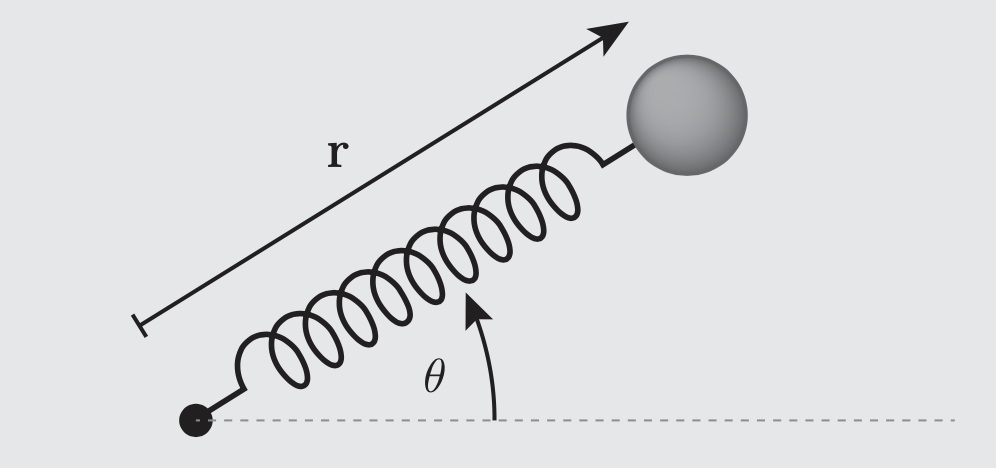
\includegraphics[width=0.5\textwidth]{PS1_P2.png}
    \label{P2}
\end{figure}

\textbf{Summary of Key Points:}

\begin{itemize}
    \item \textbf{1. Decompose the Equation of Motion:}
    Start with Newton's Second Law, $\mathbf{F} = m\mathbf{a}$. By substituting the force $\mathbf{F} = -k(x\hat{i} + y\hat{j})$ and acceleration $\mathbf{a} = \ddot{x}\hat{i} + \ddot{y}\hat{j}$, the vector equation is separated into two independent components: $m\ddot{x} + kx = 0$ and $m\ddot{y} + ky = 0$.

    \item \textbf{2. Solve for $x(t)$ and $y(t)$:}
    Recognize both component equations as describing Simple Harmonic Motion. Their general solutions are $x(t) = A \cos(\omega t) + B \sin(\omega t)$ and $y(t) = C \cos(\omega t) + D \sin(\omega t)$, where the angular frequency is $\omega = \sqrt{k/m}$.

    \item \textbf{3. Calculate the Torque:}
    To show angular momentum is conserved, we must prove the net torque $\tau$ is zero. Using the definition $\tau = \mathbf{r} \times \mathbf{F}$, substitute the given force to get $\tau = \mathbf{r} \times (-k\mathbf{r})$.

    \item \textbf{4. Apply the Cross Product Identity:}
    The expression simplifies to $\tau = -k(\mathbf{r} \times \mathbf{r})$. Since the cross product of any vector with itself ($\mathbf{r} \times \mathbf{r}$) is always zero, the net torque $\tau$ is zero, which proves that angular momentum ($\mathbf{L}$) is conserved because $\tau = d\mathbf{L}/dt$.
\end{itemize}

\hrulefill

\textbf{Detailed Answer:}

\subsection*{Part 1: Deriving the Motion $x(t)$ and $y(t)$}

\begin{enumerate}
    \item \textbf{Start with Newton's Second Law:} The motion of the particle is governed by Newton's Second Law, $\textbf{F} = m\textbf{a}$.

    \item \textbf{Express in Cartesian Coordinates:} We can write the force $\textbf{F}$, position $\textbf{r}$, and acceleration $\textbf{a}$ vectors in terms of their $x$ and $y$ components:
    \begin{itemize}
        \item $\textbf{F} = -k\textbf{r} = -k(x\hat{i} + y\hat{j}) = (-kx)\hat{i} + (-ky)\hat{j}$
        \item $\textbf{a} = \frac{d^2\textbf{r}}{dt^2} = \frac{d^2x}{dt^2}\hat{i} + \frac{d^2y}{dt^2}\hat{j} = \ddot{x}\hat{i} + \ddot{y}\hat{j}$
    \end{itemize}

    \item \textbf{Set up the Equations of Motion:} By substituting these into $\textbf{F} = m\textbf{a}$, we get:
    $$(-kx)\hat{i} + (-ky)\hat{j} = m(\ddot{x}\hat{i} + \ddot{y}\hat{j})$$

    \item \textbf{Separate the Components:} For this vector equation to be true, the components in each direction ($\hat{i}$ and $\hat{j}$) must be equal. This gives us two independent scalar differential equations:
    \begin{itemize}
        \item \textbf{$x$-component:} $-kx = m\ddot{x} \implies m\ddot{x} + kx = 0$
        \item \textbf{$y$-component:} $-ky = m\ddot{y} \implies m\ddot{y} + ky = 0$
    \end{itemize}

    \item \textbf{Solve the Differential Equations:} Both equations are in the standard form for \textbf{Simple Harmonic Motion (SHM)}: $\ddot{q} + \omega^2 q = 0$.
    \begin{itemize}
        \item We can rewrite our equations as:
        \begin{itemize}
            \item $\ddot{x} + \left(\frac{k}{m}\right)x = 0$
            \item $\ddot{y} + \left(\frac{k}{m}\right)y = 0$
        \end{itemize}
        \item Let's define the \textbf{angular frequency} $\omega$ as $\omega = \sqrt{\frac{k}{m}}$.
        \item The general solution for this type of differential equation is a sum of sine and cosine functions.
    \end{itemize}

    \item \textbf{General Solution for $x(t)$ and $y(t)$:} The motion of the particle is described by:
    $$x(t) = A \cos(\omega t) + B \sin(\omega t)$$
    $$y(t) = C \cos(\omega t) + D \sin(\omega t)$$
    where $\omega = \sqrt{k/m}$.

    The four constants $A, B, C, \text{and } D$ are determined by the particle's initial position ($x_0, y_0$) and initial velocity ($v_{x0}, v_{y0}$) at $t=0$. The path of the particle is, in general, an ellipse centered at the origin.
\end{enumerate}

\hrulefill

\subsection*{Part 2: Showing Angular Momentum is Conserved}

\begin{enumerate}
    \item \textbf{Definition of Torque and Angular Momentum:} The rate of change of angular momentum $\textbf{L}$ is equal to the net external torque $\tau$ acting on the particle.
    $$\tau = \frac{d\textbf{L}}{dt}$$
    To show that angular momentum is conserved, we must show that its time derivative is zero. This means we must show that the net torque $\tau$ is zero.

    \item \textbf{Calculate the Torque:} The torque on the particle about the origin is defined as:
    $$\tau = \textbf{r} \times \textbf{F}$$
    where $\textbf{r}$ is the position vector and $\textbf{F}$ is the force.

    \item \textbf{Substitute the Force:} We are given that the force is $\textbf{F} = -k\textbf{r}$. Substituting this into the torque equation:
    $$\tau = \textbf{r} \times (-k\textbf{r})$$

    \item \textbf{Simplify the Expression:} We can pull the scalar constant $-k$ out of the cross product:
    $$\tau = -k (\textbf{r} \times \textbf{r})$$

    \item \textbf{Use the Cross Product Identity:} A fundamental property of the vector cross product is that the cross product of any vector with itself is zero. This is because the angle between $\textbf{r}$ and $\textbf{r}$ is $0^\circ$, and $\sin(0^\circ) = 0$.
    $$\textbf{r} \times \textbf{r} = 0$$

    \item \textbf{Conclusion:} Therefore, the torque on the particle is:
    $$\tau = -k(0) = 0$$

    Since the net torque is zero, the rate of change of angular momentum is also zero:
    $$\frac{d\textbf{L}}{dt} = 0$$
    This proves that the angular momentum $\textbf{L}$ is a constant value and is \textbf{conserved}. This is a general property of all \textbf{central forces} (forces that always point along the $\textbf{r}$ vector).
\end{enumerate}

\newpage
\section*{Projectile with drag [15 points]} 
Consider a projectile subject to a drag force $\textbf{F}=-m\alpha \textbf{v}$. If it is fired
with speed $v_0$ at an angle $\theta$, it can be shown that the height as a function of time is given by 
\begin{equation}
    y(t) = \frac{1}{\alpha} \left( v_0 \sin \theta + \frac{g}{\alpha} \right) \left( 1 - e^{-\alpha t} \right) - \frac{g t}{\alpha}.
\end{equation}
Show that this reduces to the usual projectile expression $y(t)=v_0(\sin\theta) t - gt^2/2$. What exactly is meant by ``small $\alpha$"? \\
Bonus question [5 points]: Derive Equation (1) using Newton's second law. 

\textbf{Summary:}

\begin{itemize}
    \item \textbf{1. Use Taylor Series Expansion:}
    To show the drag equation reduces to the no-drag case, the term $e^{-\alpha t}$ is expanded using a Taylor series ($e^x \approx 1 + x + x^2/2$). This is necessary because directly substituting $\alpha = 0$ leaves the equation undefined.

    \item \textbf{2. Substitute and Simplify:}
    Substituting the expansion $1 - e^{-\alpha t} \approx \alpha t - \frac{1}{2}\alpha^2 t^2$ into the given $y(t)$ equation allows for algebraic cancellation of the $\frac{1}{\alpha}$ terms. Taking the limit as $\alpha \to 0$ then leaves the standard projectile equation $y(t) = (v_0 \sin \theta) t - \frac{1}{2}gt^2$.

    \item \textbf{3. Define "Small $\alpha$":}
    The "small $\alpha$" approximation is valid only when the exponent $\alpha t \ll 1$. This physically means the damping coefficient $\alpha$ (in 1/s) must be small relative to the reciprocal of the time $t$ over which the motion is observed.

    \item \textbf{4. Derive $y(t)$ (Bonus):}
    The $y(t)$ equation is derived by setting up Newton's second law for the vertical ($y$) forces, $m\ddot{y} = -mg - m\alpha v_y$. This differential equation is solved twice: first by separating variables to find $v_y(t)$, and a second time by integrating $v_y(t)$ to find $y(t)$, applying the initial conditions $y(0) = 0$ and $v_y(0) = v_0 \sin \theta$ to find the constants.
\end{itemize}

\hrulefill

\textbf{Detailed Answer:}

\subsection*{Part 1: Reduction to the No-Drag Case (Small $\alpha$)}

We are given the equation for the height $y(t)$:
$$y(t) = \frac{1}{\alpha} \left( v_0 \sin \theta + \frac{g}{\alpha} \right) \left( 1 - e^{-\alpha t} \right) - \frac{g t}{\alpha}$$
We need to show that this reduces to the standard projectile equation $y(t)=v_0(\sin\theta) t - \frac{1}{2}gt^2$ when $\alpha$ is small.

\begin{enumerate}
    \item \textbf{Identify the Problem Term:} If we simply set $\alpha = 0$, the expression is undefined due to $\alpha$ in the denominator. This indicates we need to use a series expansion for the limit $\alpha \to 0$.

    \item \textbf{Use the Taylor Series Expansion:} The key term is $e^{-\alpha t}$. We can expand this using the Taylor (or Maclaurin) series for $e^x$ around $x=0$, where $x = -\alpha t$.
    $$e^x = 1 + x + \frac{x^2}{2!} + \frac{x^3}{3!} + \dots$$
    Substituting $x = -\alpha t$:
    $$e^{-\alpha t} = 1 + (-\alpha t) + \frac{(-\alpha t)^2}{2} + \frac{(-\alpha t)^3}{6} + \dots$$
    $$e^{-\alpha t} = 1 - \alpha t + \frac{\alpha^2 t^2}{2} - \frac{\alpha^3 t^3}{6} + \dots$$
    For "small $\alpha$", we only need to keep terms up to $\alpha^2$, as we will see.

    \item \textbf{Substitute the Expansion:} Let's substitute this series into the $(1 - e^{-\alpha t})$ part of the equation:
    $$1 - e^{-\alpha t} = 1 - \left( 1 - \alpha t + \frac{\alpha^2 t^2}{2} - O(\alpha^3) \right)$$
    $$1 - e^{-\alpha t} = \alpha t - \frac{\alpha^2 t^2}{2} + O(\alpha^3)$$
    (Here, $O(\alpha^3)$ means "terms of order $\alpha^3$ or higher.")

    \item \textbf{Substitute Back into $y(t)$:}
    $$y(t) = \frac{1}{\alpha} \left( v_0 \sin \theta + \frac{g}{\alpha} \right) \left( \alpha t - \frac{\alpha^2 t^2}{2} + \dots \right) - \frac{g t}{\alpha}$$

    \item \textbf{Expand the Brackets:} We will distribute the terms.
    $$y(t) = \left[ \frac{1}{\alpha} (v_0 \sin \theta) \left( \alpha t - \frac{\alpha^2 t^2}{2} + \dots \right) \right] + \left[ \frac{1}{\alpha} \left(\frac{g}{\alpha}\right) \left( \alpha t - \frac{\alpha^2 t^2}{2} + \dots \right) \right] - \frac{g t}{\alpha}$$
    
    \begin{itemize}
        \item \textbf{First term:}
        $$\frac{v_0 \sin \theta}{\alpha} \left( \alpha t - \frac{\alpha^2 t^2}{2} + \dots \right) = (v_0 \sin \theta) t - (v_0 \sin \theta) \frac{\alpha t^2}{2} + \dots$$
        \item \textbf{Second term:}
        $$\frac{g}{\alpha^2} \left( \alpha t - \frac{\alpha^2 t^2}{2} + \dots \right) = \frac{g t}{\alpha} - \frac{g t^2}{2} + \dots$$
    \end{itemize}

    \item \textbf{Combine and Simplify:} Now, let's put all the pieces back together:
    $$y(t) = \left( (v_0 \sin \theta) t - (v_0 \sin \theta) \frac{\alpha t^2}{2} + \dots \right) + \left( \frac{g t}{\alpha} - \frac{g t^2}{2} + \dots \right) - \frac{g t}{\alpha}$$
    Notice that the $\frac{g t}{\alpha}$ terms cancel each other out:
    $$y(t) = (v_0 \sin \theta) t - (v_0 \sin \theta) \frac{\alpha t^2}{2} - \frac{g t^2}{2} + O(\alpha^2)$$

    \item \textbf{Take the Limit:} In the limit as $\alpha \to 0$, all terms that still contain $\alpha$ (like the $(v_0 \sin \theta) \frac{\alpha t^2}{2}$ term) will go to zero.
    $$\lim_{\alpha \to 0} y(t) = (v_0 \sin \theta) t - \frac{g t^2}{2}$$
    This is exactly the standard expression for projectile motion without drag.
\end{enumerate}

\hrulefill

\subsection*{Part 2: What is meant by "small $\alpha$"?}

The approximation we used was a Taylor expansion of $e^{-\alpha t}$. This type of expansion is only valid when the exponent, $\alpha t$, is small.

\textbf{"Small $\alpha$" means that the product $\alpha t$ is much less than 1 (i.e., $\alpha t \ll 1$).}

\begin{itemize}
    \item \textbf{Physical Interpretation:} $\alpha$ has units of 1/time (it's a damping coefficient). The variable $t$ is the time of flight. Therefore, "small $\alpha$" means that the damping coefficient is much smaller than the reciprocal of the time of interest.
    \item \textbf{Mathematical Justification:} Our approximation $e^{-\alpha t} \approx 1 - \alpha t + \frac{1}{2}(\alpha t)^2$ is only accurate if the higher-order terms, like $(\alpha t)^3$, are negligible. This condition is met only if the magnitude of the exponent, $|\alpha t|$, is small.
    \item \textbf{In short:} $\alpha$ isn't just small in an absolute sense; it must be small \textit{relative to the time $t$} over which we are observing the motion. If the time $t$ is very large, $\alpha$ must be \textit{even smaller} for the no-drag approximation to hold.
\end{itemize}

\hrulefill

\subsection*{Bonus: Derive Equation (1)}

\begin{enumerate}
    \item \textbf{Newton's Second Law:} We start with $\textbf{F}_{net} = m\textbf{a}$. The forces acting on the projectile are gravity ($\textbf{F}_g$) and drag ($\textbf{F}_D$).
    \begin{itemize}
        \item $\textbf{F}_g = -mg \hat{j}$
        \item $\textbf{F}_D = -m\alpha \textbf{v} = -m\alpha (v_x \hat{i} + v_y \hat{j})$
        \item $\textbf{a} = \ddot{x} \hat{i} + \ddot{y} \hat{j}$
    \end{itemize}

    \item \textbf{Set up the Vector Equation:}
    $$\textbf{F}_{net} = \textbf{F}_g + \textbf{F}_D = (-mg \hat{j}) + (-m\alpha v_x \hat{i} - m\alpha v_y \hat{j})$$
    $$m(\ddot{x} \hat{i} + \ddot{y} \hat{j}) = (-m\alpha v_x) \hat{i} + (-mg - m\alpha v_y) \hat{j}$$

    \item \textbf{Separate Components:} We are only interested in the vertical motion for $y(t)$.
    \begin{itemize}
        \item \textbf{$y$-component:} $m\ddot{y} = -mg - m\alpha v_y$
    \end{itemize}
    Dividing by $m$ and writing $\ddot{y}$ as $\frac{dv_y}{dt}$:
    $$\frac{dv_y}{dt} = -g - \alpha v_y$$

    \item \textbf{Solve the Differential Equation for $v_y(t)$:} This is a first-order, separable differential equation.
    $$\frac{dv_y}{g + \alpha v_y} = -dt$$
    Integrate both sides:
    $$\int \frac{dv_y}{g + \alpha v_y} = \int -dt$$
    $$\frac{1}{\alpha} \ln(g + \alpha v_y) = -t + C_1$$
    (We use $g + \alpha v_y$ instead of $|g + \alpha v_y|$ assuming it remains positive, which it does until it reaches terminal velocity $-g/\alpha$).
    
    Solve for $v_y$:
    $$\ln(g + \alpha v_y) = -\alpha t + \alpha C_1$$
    $$g + \alpha v_y = e^{-\alpha t + \alpha C_1} = e^{\alpha C_1} e^{-\alpha t}$$
    Let $A = e^{\alpha C_1}$ be our new constant of integration.
    $$\alpha v_y = A e^{-\alpha t} - g$$
    $$v_y(t) = \frac{A}{\alpha} e^{-\alpha t} - \frac{g}{\alpha}$$

    \item \textbf{Apply Initial Condition for $v_y(0)$:} At $t=0$, the initial vertical velocity is $v_y(0) = v_0 \sin \theta$.
    $$v_0 \sin \theta = \frac{A}{\alpha} e^0 - \frac{g}{\alpha} = \frac{A}{\alpha} - \frac{g}{\alpha}$$
    $$A = \alpha v_0 \sin \theta + g = \alpha \left( v_0 \sin \theta + \frac{g}{\alpha} \right)$$

    \item \textbf{Substitute $A$ to find $v_y(t)$:}
    $$v_y(t) = \frac{\alpha (v_0 \sin \theta + g/\alpha)}{\alpha} e^{-\alpha t} - \frac{g}{\alpha}$$
    $$v_y(t) = \left( v_0 \sin \theta + \frac{g}{\alpha} \right) e^{-\alpha t} - \frac{g}{\alpha}$$

    \item \textbf{Find $y(t)$ by Integrating $v_y(t)$:} Now we integrate $v_y(t) = \frac{dy}{dt}$ with respect to time.
    $$y(t) = \int v_y(t) dt = \int \left[ \left( v_0 \sin \theta + \frac{g}{\alpha} \right) e^{-\alpha t} - \frac{g}{\alpha} \right] dt$$
    $$y(t) = \left( v_0 \sin \theta + \frac{g}{\alpha} \right) \left( -\frac{1}{\alpha} e^{-\alpha t} \right) - \frac{g t}{\alpha} + C_2$$

    \item \textbf{Apply Initial Condition for $y(0)$:} At $t=0$, the initial height is $y(0) = 0$.
    $$0 = \left( v_0 \sin \theta + \frac{g}{\alpha} \right) \left( -\frac{1}{\alpha} e^0 \right) - \frac{g(0)}{\alpha} + C_2$$
    $$0 = -\frac{1}{\alpha} \left( v_0 \sin \theta + \frac{g}{\alpha} \right) + C_2$$
    $$C_2 = \frac{1}{\alpha} \left( v_0 \sin \theta + \frac{g}{\alpha} \right)$$

    \item \textbf{Substitute $C_2$ to find the Final $y(t)$:}
    $$y(t) = \left( v_0 \sin \theta + \frac{g}{\alpha} \right) \left( -\frac{1}{\alpha} e^{-\alpha t} \right) - \frac{g t}{\alpha} + \frac{1}{\alpha} \left( v_0 \sin \theta + \frac{g}{\alpha} \right)$$
    We can factor out the common term $\frac{1}{\alpha} \left( v_0 \sin \theta + \frac{g}{\alpha} \right)$:
    $$y(t) = \frac{1}{\alpha} \left( v_0 \sin \theta + \frac{g}{\alpha} \right) \left( 1 - e^{-\alpha t} \right) - \frac{g t}{\alpha}$$
    This matches Equation (1) exactly.
\end{enumerate}

\newpage 
\section*{Potential energies for positive power-law forces [15 points]} 
A particle moves in one dimension subject to the power-law force $F=-kx^n$, where the coefficient $k$ is positive, and $n$ is a positive integer. Please find the potential energy of the particle and also the maximum distance $x_{\rm max}$ it can reach from the origin, in terms of its maximum speed $v_{\rm max}$. The maximum distance is the \textbf{turning point} of the particle, because as the particle approaches this position it slows down, stops at $x_{\rm max}$, and turns around and heads in the opposite direction.

\textbf{Answer:}

\subsection*{Part 1: Finding the Potential Energy $U(x)$}

\begin{enumerate}
    \item \textbf{Definition of Potential Energy:} The potential energy $U(x)$ is related to the conservative force $F(x)$ by the definition $F(x) = -\frac{dU(x)}{dx}$. To find the potential energy, we must integrate this relationship:
    $$U(x) = - \int F(x) dx + C$$
    where $C$ is the constant of integration.

    \item \textbf{Substitute the Force:} We are given the force $F(x) = -kx^n$.
    $$U(x) = - \int (-kx^n) dx + C$$
    $$U(x) = k \int x^n dx + C$$

    \item \textbf{Perform the Integration:} Using the power rule for integration $\int x^n dx = \frac{x^{n+1}}{n+1}$:
    $$U(x) = k \left( \frac{x^{n+1}}{n+1} \right) + C$$

    \item \textbf{Set the Reference Point:} We are free to choose a reference point where the potential energy is zero. A convenient choice for this problem is to set the potential energy to zero at the origin ($x=0$).
    $$U(0) = 0$$
    $$k \left( \frac{0^{n+1}}{n+1} \right) + C = 0 \implies C = 0$$
    
    (Note: Since $n$ is a positive integer, $n+1 \ge 2$, so $0^{n+1}$ is well-defined and equal to 0).

    \item \textbf{Final Expression for $U(x)$:} With $C=0$, the potential energy of the particle is:
    $$U(x) = \frac{k}{n+1} x^{n+1}$$
\end{enumerate}

\hrulefill

\subsection*{Part 2: Finding the Maximum Distance $x_{\rm max}$}

\begin{enumerate}
    \item \textbf{Conservation of Energy:} The force is conservative (it only depends on position), so the total mechanical energy $E$ of the particle is conserved. The total energy is the sum of the kinetic energy $K$ and the potential energy $U$.
    $$E = K + U = \frac{1}{2}mv^2 + \frac{k}{n+1}x^{n+1} = \text{Constant}$$

    \item \textbf{Identify Key Points:} We can analyze the energy of the particle at two critical points in its motion:
    \begin{itemize}
        \item \textbf{At $x=0$ (the origin):} The potential energy $U(0) = 0$. Since the total energy $E = K + U$ is constant, the kinetic energy $K$ must be at its maximum when the potential energy $U$ is at its minimum. Therefore, the particle reaches its \textbf{maximum speed $v_{\rm max}$} as it passes through the origin.
        \item \textbf{At $x=x_{\rm max}$ (the turning point):} The problem defines this as the \textbf{maximum distance}, where the particle stops and turns around. At this point, its speed is momentarily zero, so $v=0$.
    \end{itemize}

    \item \textbf{Write the Energy Equation for Both Points:}
    \begin{itemize}
        \item \textbf{Energy at $x=0$:}
        $$E = K_{\text{max}} + U(0) = \frac{1}{2}m v_{\rm max}^2 + 0$$
        $$E = \frac{1}{2}m v_{\rm max}^2$$

        \item \textbf{Energy at $x=x_{\rm max}$:}
        $$E = K_{\text{turning}} + U(x_{\rm max}) = \frac{1}{2}m(0)^2 + \frac{k}{n+1} (x_{\rm max})^{n+1}$$
        $$E = \frac{k}{n+1} (x_{\rm max})^{n+1}$$
    \end{itemize}

    \item \textbf{Equate the Energies:} Since total energy $E$ is conserved, we can set the energy at $x=0$ equal to the energy at $x=x_{\rm max}$:
    $$\frac{1}{2}m v_{\rm max}^2 = \frac{k}{n+1} (x_{\rm max})^{n+1}$$

    \item \textbf{Solve for $x_{\rm max}$:} We now isolate the $x_{\rm max}$ term.
    $$(x_{\rm max})^{n+1} = \frac{n+1}{k} \left( \frac{1}{2}m v_{\rm max}^2 \right)$$
    $$(x_{\rm max})^{n+1} = \frac{m(n+1)}{2k} v_{\rm max}^2$$

    Finally, we take the $(n+1)$-th root of both sides to get the maximum distance:
    $$x_{\rm max} = \left( \frac{m(n+1)v_{\rm max}^2}{2k} \right)^{\frac{1}{n+1}}$$
\end{enumerate}

\newpage 
\section*{Problems from Classical Mechanics of John R. Taylor [110 points]} 
Chapter 1: 1.27, 1.46, 1.37, 1.47 [10$\times3$ + 15 points]\\
Chapter 4: 4.2, 4.3, 4.21, 4.23, 4.27, 4.25 [$10\times5$ + 15 points]\\

\newpage
\subsection*{1.27}
The hallmark of an inertial reference frame is that any object which is subject to zero net force will travel in a straight line at constant speed. To illustrate this, consider the following experiment: I am standing on the ground (which we shall take to be an inertial frame) beside a perfectly flat horizontal turntable, rotating with constant angular velocity $\omega$. I lean over and shove a frictionless puck so that it slides across the turntable, straight through the center. The puck is subject to zero net force and, as seen from my inertial frame, travels in a straight line. Describe the puck’s path as observed by someone sitting at rest on the turntable. This requires careful thought, but you should be able to get a qualitative picture. For a quantitative picture, it helps to use polar coordinates; see Problem 1.46.

\textbf{Answer}:

\begin{enumerate}
    \item \textbf{Motion in the Inertial Frame (Seen from the Ground)}
    \begin{itemize}
        \item The puck is frictionless, so the net force on it is zero.
        \item From the ground frame, its path is a \textbf{straight line at a constant speed}, $v_0$.
        \item As shown in the left figure, the puck is launched from point \textbf{A} at $t=0$. It travels "due west" (in the inertial frame), passes through the center \textbf{O}, and flies off the table at point \textbf{C}.
        \item The total time for this crossing is $T = \text{distance} / \text{speed} = 2R / v_0$, where $R$ is the radius of the turntable.
    \end{itemize}
    
    

    \item \textbf{Motion in the Rotating Frame (Seen from the Turntable)}
    
    We now analyze the motion from the perspective of an observer sitting on the rotating turntable at point \textbf{A}. The turntable rotates counter-clockwise (A toward B) with a constant angular velocity $\omega$.
    
    \begin{itemize}
        \item \textbf{Initial Velocity:} We must find the puck's velocity *relative to the observer* at $t=0$.
        \begin{itemize}
            \item \textbf{Puck's Inertial Velocity ($\mathbf{v}_p$):} The puck is moving "west" with speed $v_0$.
            \item \textbf{Observer's Inertial Velocity ($\mathbf{v}_{obs}$):} The observer at A is rotating "north" (in the direction of B) with a tangential speed of $\omega R$.
            \item \textbf{Relative Velocity ($\mathbf{v}_{rel}$):} The velocity seen by the observer is $\mathbf{v}_{rel} = \mathbf{v}_p - \mathbf{v}_{obs}$. This is the vector sum of a "west" component ($v_0$) and a "south" component ($\omega R$).
            \item Therefore, the observer at A sees the puck *initially* move away from them both \textbf{west and south}.
        \end{itemize}

        \item \textbf{Curved Path:} As the puck moves inward toward the center O, it travels over parts of the turntable that are moving "north" *slower* than point A (the tangential speed of the table at a radius $r$ is only $\omega r$). Because the "northward" velocity of the floor beneath the puck is decreasing, the "southward" component of the puck's relative velocity changes, causing the path to \textbf{curve to the right} (in the southerly direction), as shown in the right figure.

        \item \textbf{Final Position:} The puck follows this curved path, passing through O, and eventually reaches the edge of the turntable. We know from the inertial frame that the puck flies off at point \textbf{C}. In the time $T = 2R/v_0$ it took for this to happen, the turntable has rotated. The point \textbf{B} on the turntable has rotated by an angle of $\theta = \omega T = \omega(2R/v_0)$ and is now located exactly where point C is in the inertial frame.
        \item Therefore, in the turntable's frame, the puck starts at \textbf{A} and ends at \textbf{B}.
    \end{itemize}
\end{enumerate}

\begin{figure}[h]
    \centering
    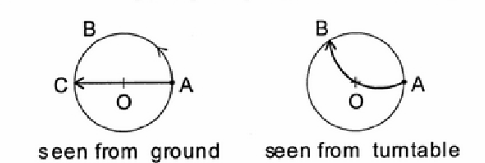
\includegraphics[width=0.5\textwidth]{1.27.png}
    \label{1.27}
    \caption{Different paths}
\end{figure}

\subsection*{Conclusion}

The observer on the non-inertial turntable sees the puck, which is subject to zero net force, follow a \textbf{curved path}. It starts at A, initially moves "west and south," and then curves "to the right" before flying off the edge at point B. This curved path is the direct result of observing motion from a rotating reference frame and would require the invention of \textbf{fictitious forces} (Coriolis and centrifugal) to be explained by Newton's laws in that frame.


\newpage
\subsection*{1.46}
Consider the experiment of Problem 1.27, in which a frictionless puck is slid straight across a rotating turntable through the center $O$. (\textbf{a}) Write down the polar coordinates $r, \phi$ of the puck as functions of time, as measured in the inertial frame $S$ of an observer on the ground. (Assume that the puck was launched along the axis $\phi = 0$ at $t = 0$) (\textbf{b}) Now write down the polar coordinates $r', \phi'$ of the puck as measured by an observer (frame $S'$) at rest on the turntable. (Choose these coordinates so that $\phi$ and $\phi'$ coincide at $t = 0$.) Describe and sketch the path seen by this second observer. Is the frame $S'$ inertial?

\textbf{Answer}:

\subsection*{Setup}
We are analyzing the motion of a frictionless puck slid across a rotating turntable.

\begin{itemize}
    \item \textbf{Frame $S$ (Inertial Frame):} This is the ground. We use polar coordinates $(r, \phi)$.
    \item \textbf{Frame $S'$ (Rotating Frame):} This is the turntable, rotating with a constant counter-clockwise angular velocity $\omega$ relative to $S$. We use polar coordinates $(r', \phi')$.
    \item \textbf{Initial Conditions:} At $t=0$, the frames are aligned ($\phi = \phi' = 0$).
    \item \textbf{The Path in $S$:} As established in the "standard answer" to the previous problem, the puck is launched at $t=0$ from the edge (point A) and travels in a straight line through the center (O) to the opposite edge (point C). We set the $\phi=0$ axis (the $x$-axis) to align with this path.
    \begin{itemize}
        \item The puck starts at $x(0) = R$, $y(0) = 0$.
        \item It has a constant velocity $\mathbf{v} = -v_0 \hat{\mathbf{i}}$.
        \item The Cartesian path in $S$ is:
        $$x(t) = R - v_0 t$$
        $$y(t) = 0$$
    \end{itemize}
\end{itemize}

\hrulefill

\section*{(a) Polar Coordinates in the Inertial Frame ($S$)}

We need to convert the Cartesian path in $S$ to polar coordinates $(r, \phi)$.

\begin{enumerate}
    \item \textbf{Radial Coordinate $r(t)$:}
    The radius $r$ is the distance from the origin.
    $$r(t) = \sqrt{x(t)^2 + y(t)^2} = \sqrt{(R - v_0 t)^2 + 0^2}$$
    $$r(t) = |R - v_0 t|$$
    This shows the puck starts at $r=R$, moves to $r=0$ (at $t=R/v_0$), and moves back out to $r=R$ (at $t=2R/v_0$).

    \item \textbf{Angular Coordinate $\phi(t)$:}
    The angle $\phi$ is measured from the positive $x$-axis. The puck's path $y(t)=0$ lies entirely on the $x$-axis.
    
    \textit{Clarification on $\phi(t)$:} The angle $\phi$ is defined by the \textit{direction} from the origin. By standard convention:
    \begin{itemize}
        \item Any point on the \textbf{positive x-axis} (where $x>0, y=0$) has an angle **$\phi = 0$**.
        \item Any point on the \textbf{negative x-axis} (where $x<0, y=0$) has an angle **$\phi = \pi$**.
    \end{itemize}
    We analyze the puck's position $x(t) = R - v_0 t$:
    \begin{itemize}
        \item \textbf{For $0 \le t < R/v_0$:}
        In this interval, $v_0 t < R$, so $x(t) = R - v_0 t$ is \textbf{positive}. The puck is on the positive $x$-axis.
        $$\phi(t) = 0$$
        \item \textbf{At $t = R/v_0$:}
        $x(t) = 0$. The puck is at the origin, and $\phi$ is undefined.
        \item \textbf{For $R/v_0 < t \le 2R/v_0$:}
        In this interval, $v_0 t > R$, so $x(t) = R - v_0 t$ is \textbf{negative}. The puck is on the negative $x$-axis.
        $$\phi(t) = \pi$$
    \end{itemize}
\end{enumerate}

So, the puck's coordinates in the inertial frame $S$ are:
$$r(t) = |R - v_0 t|$$
$$\phi(t) = \begin{cases} 0 & \text{if } 0 \le t < R/v_0 \\ \pi & \text{if } R/v_0 < t \le 2R/v_0 \end{cases}$$

\hrulefill

\section*{(b) Polar Coordinates in the Rotating Frame ($S'$)}

Now we find the coordinates $(r', \phi')$ for the observer on the turntable.

\begin{enumerate}
    \item \textbf{Radial Coordinate $r'(t)$:}
    The origin of $S'$ is the same as $S$. Therefore, the radial distance from the origin is the same in both frames.
    $$r'(t) = r(t) = |R - v_0 t|$$

    \item \textbf{Angular Coordinate $\phi'(t)$:}
    The frame $S'$ rotates with angular velocity $\omega$. At time $t$, its $\phi'=0$ axis has rotated by an angle $\theta_{\text{rot}} = \omega t$ relative to the $\phi=0$ axis of $S$.
    The relationship between the angles is:
    $$\phi_{\text{puck in S}} = \phi'_{\text{puck in S'}} + \theta_{\text{rotation of S'}}$$
    $$\phi(t) = \phi'(t) + \omega t$$
    Solving for $\phi'(t)$:
    $$\phi'(t) = \phi(t) - \omega t$$
    
    We now use our result for $\phi(t)$ from part (a):
    \begin{itemize}
        \item \textbf{For $0 \le t < R/v_0$:}
        $$\phi'(t) = 0 - \omega t = -\omega t$$
        \item \textbf{For $R/v_0 < t \le 2R/v_0$:}
        $$\phi'(t) = \pi - \omega t$$
    \end{itemize}
\end{enumerate}

So, the puck's coordinates in the rotating frame $S'$ are:
$$r'(t) = |R - v_0 t|$$
$$\phi'(t) = \begin{cases} -\omega t & \text{if } 0 \le t < R/v_0 \\ \pi - \omega t & \text{if } R/v_0 < t \le 2R/v_0 \end{cases}$$

\hrulefill

\subsection*{Path Description and Sketch}

\begin{itemize}
    \item \textbf{Description:} The observer in $S'$ sees the puck start at $t=0$ at $(r', \phi') = (R, 0)$.
    \begin{enumerate}
        \item \textbf{Path In ($0 \le t < R/v_0$):} As $t$ increases, the radius $r' = R - v_0 t$ decreases linearly. The angle $\phi' = -\omega t$ becomes increasingly negative (i.e., it moves clockwise). The puck follows a \textbf{clockwise spiral inward}, reaching the origin $O$ at $t = R/v_0$.
        \item \textbf{Path Out ($R/v_0 < t \le 2R/v_0$):} Just after passing the origin, the radius $r' = v_0 t - R$ increases linearly. The angle $\phi'(t) = \pi - \omega t$ continues its clockwise motion (becoming more negative). The puck follows a \textbf{clockwise spiral outward} from the origin.
    \end{enumerate}
    The path passes directly through the origin, which is why the angle $\phi'$ effectively jumps by $\pi$ at $t=R/v_0$. The overall path is a two-part spiral.

    \item \textbf{Sketch:}
    The path seen by the observer on the turntable starts at point A ($r'=R, \phi'=0$) and spirals inward to the origin O in a clockwise direction. It then passes through O and spirals outward, still moving clockwise, until it reaches the edge of the table at a new point B.

    
\end{itemize}

\subsection*{Is the frame $S'$ inertial?}

\textbf{No, the frame $S'$ is not an inertial frame.}

An inertial frame is one in which Newton's First Law holds: an object with zero net force moves in a straight line at a constant velocity.

In this problem, the puck is frictionless, so the net force on it is \textbf{zero}. However, the observer in frame $S'$ sees the puck follow a \textbf{curved spiral path}, not a straight line. Since Newton's First Law is violated, the frame $S'$ is non-inertial.

\newpage
\subsection*{1.37}

A student kicks a frictionless puck with initial speed $v_0$, so that it slides straight up a plane that is inclined at an angle $\theta$ about the horizontal. (a) Write down Newton's second law for the puck and solve to give its position as a function of time. (b) How long will the puck take to return to its starting point?

\subsection*{(a) Newton's Second Law and Position $x(t)$}

\begin{enumerate}
    \item \textbf{Free-Body Diagram and Coordinate System:}
    \begin{itemize}
        \item We set up a coordinate system with the $x$-axis pointing \textbf{up the incline} (parallel to the puck's motion) and the $y$-axis pointing \textbf{perpendicular} to the incline, away from the surface. The origin $x=0$ is the puck's starting point.
        \item There are two forces acting on the puck:
        \begin{enumerate}
            \item \textbf{Normal Force ($N$):} Acts perpendicular to the surface, entirely in the $+y$ direction.
            \item \textbf{Gravity ($mg$):} Acts vertically downwards.
        \end{enumerate}
        \item We must resolve the force of gravity into components parallel ($x$) and perpendicular ($y$) to the incline. The angle between the vertical gravitational force and our $y$-axis is $\theta$.
        \begin{itemize}
            \item $W_x$ (parallel component): $-mg \sin\theta$ (points down the incline, in the $-x$ direction)
            \item $W_y$ (perpendicular component): $-mg \cos\theta$ (points into the incline, in the $-y$ direction)
        \end{itemize}
    \end{itemize}

    \item \textbf{Applying Newton's Second Law ($\Sigma \textbf{F} = m\textbf{a}$):}
    \begin{itemize}
        \item We separate the forces into their $x$ and $y$ components. The puck only moves along the $x$-axis, so its acceleration $a_y$ is 0.
        \item \textbf{$y$-direction:}
        $$\Sigma F_y = N - mg \cos\theta = m a_y = 0$$
        $$N = mg \cos\theta$$
        (This confirms the normal force, but is not needed to find the position).

        \item \textbf{$x$-direction:} This is the equation of motion along the incline.
        $$\Sigma F_x = -mg \sin\theta = m a_x$$
    \end{itemize}

    \item \textbf{Solving for Acceleration:}
    \begin{itemize}
        \item By dividing by $m$, we find the puck's constant acceleration:
        $$a_x = -g \sin\theta$$
        \item The negative sign correctly indicates that the acceleration is constant and directed \textit{down} the incline, opposing the initial velocity.
    \end{itemize}

    \item \textbf{Solving for Position $x(t)$:}
    \begin{itemize}
        \item We use the standard kinematic equation for position under constant acceleration $a$:
        $$x(t) = x_0 + v_0 t + \frac{1}{2} a t^2$$
        \item We substitute our known values:
        \begin{itemize}
            \item $x_0 = 0$ (it starts at the origin)
            \item $v_0 = v_0$ (this is the given initial speed, in the $+x$ direction)
            \item $a = -g \sin\theta$
        \end{itemize}
        \item Plugging these in gives the position as a function of time:
        $$x(t) = v_0 t - \frac{1}{2} (g \sin\theta) t^2$$
    \end{itemize}
\end{enumerate}

\hrulefill

\subsection*{(b) Time to Return to Starting Point}

\begin{enumerate}
    \item \textbf{Set Up the Equation:}
    \begin{itemize}
        \item The puck starts at $x=0$. It returns to its starting point when its position $x(t)$ is once again equal to $0$.
        \item We use the position function from part (a) and set $x(t) = 0$:
        $$0 = v_0 t - \frac{1}{2} (g \sin\theta) t^2$$
    \end{itemize}

    \item \textbf{Solve for $t$:}
    \begin{itemize}
        \item We can find the solutions for $t$ by factoring the equation:
        $$0 = t \left( v_0 - \frac{1}{2} (g \sin\theta) t \right)$$
        \item This equation has two possible solutions:
        \begin{enumerate}
            \item \textbf{$t = 0$:} This is the trivial solution, representing the moment the puck \textit{starts} at the origin.
            \item \textbf{$v_0 - \frac{1}{2} (g \sin\theta) t = 0$:} This is the non-trivial solution we are looking for.
        \end{enumerate}
    \end{itemize}

    \item \textbf{Isolate $t$:}
    \begin{itemize}
        \item We solve the second equation for $t$:
        $$v_0 = \frac{1}{2} (g \sin\theta) t$$
        $$t = \frac{2 v_0}{g \sin\theta}$$
        \item This is the total time the puck will take to go up the incline, stop, and slide back down to its starting point.
    \end{itemize}
\end{enumerate}

\newpage
\subsection*{1.47}

Let the position of a point $P$ in three dimensions be given by the vector $\mathbf{r} = (x,y,z)$ in rectangular (or Cartesian) coordinates. The same position can be specified by \textbf{cylindrical polar coordinates}, $\rho, \phi, z$, which are defined as follows: Let $P'$ denote the projection of P onto the $xy$ plane; that is, $P'$ has Cartesian coordinates $(x,y,0)$. Then $\rho$ and $\phi$ are defined as the two-dimensional polar coordinates of $P'$ in the $xy$ plane, while $z$ is the third Cartesian coordinate, unchanged. (\textbf{a}) Make a sketch to illustrate the three cylindrical coordinates. Give expressions for $\rho, \phi, z$ in terms of the Cartesian coordinates $x,y,z$. Explain in words what $\rho$ is ("$\rho$ is the distance of $P$ from XX?"). There are many variants in notation. For instance, some people use $r$ instead of $\rho$. Explain why this use of $r$ is unfortunate. (\textbf{b}) Describe the three unit vectors $\hat{\rho}, \hat{\phi}, \hat{\mathbf{z}}$ and write the expansion of the position vector $\mathbf{r}$ in terms of these unit vectors. (\textbf{c}) Differentiate your last answer twice to find the cylindrical components of the acceleration $a = \ddot{\mathbf{r}}$ of the particle. To do this, you will need to know the time derivatives of $\hat{\rho}$ and $\hat{\phi}$. You could get these from the corresponding two-dimensional results (1.42) and (1.46), or you could derive them directly as in Problem 1.48.

\textbf{Answer}:

\subsection*{(a) Sketch, Coordinates, and Notation}

\begin{enumerate}
    \item \textbf{Sketch: (Fig.~\ref{coord})}
    \begin{itemize}
        \item We start with the 3D Cartesian axes ($x, y, z$).
        \item A point $P$ has coordinates $(x, y, z)$.
        \item We project $P$ straight down onto the $xy$-plane to get the point $P'$, which has coordinates $(x, y, 0)$.
        \item The coordinate $z$ is the height of $P$ above the $xy$-plane (the length of the segment $P'P$).
        \item The coordinate $\rho$ (rho) is the distance from the origin $O$ to the projection $P'$. It is the radial distance in the $xy$-plane.
        \item The coordinate $\phi$ (phi) is the angle in the $xy$-plane, measured counter-clockwise from the positive $x$-axis to the line segment $OP'$.
    \end{itemize}

\begin{figure}[h]
    \centering
    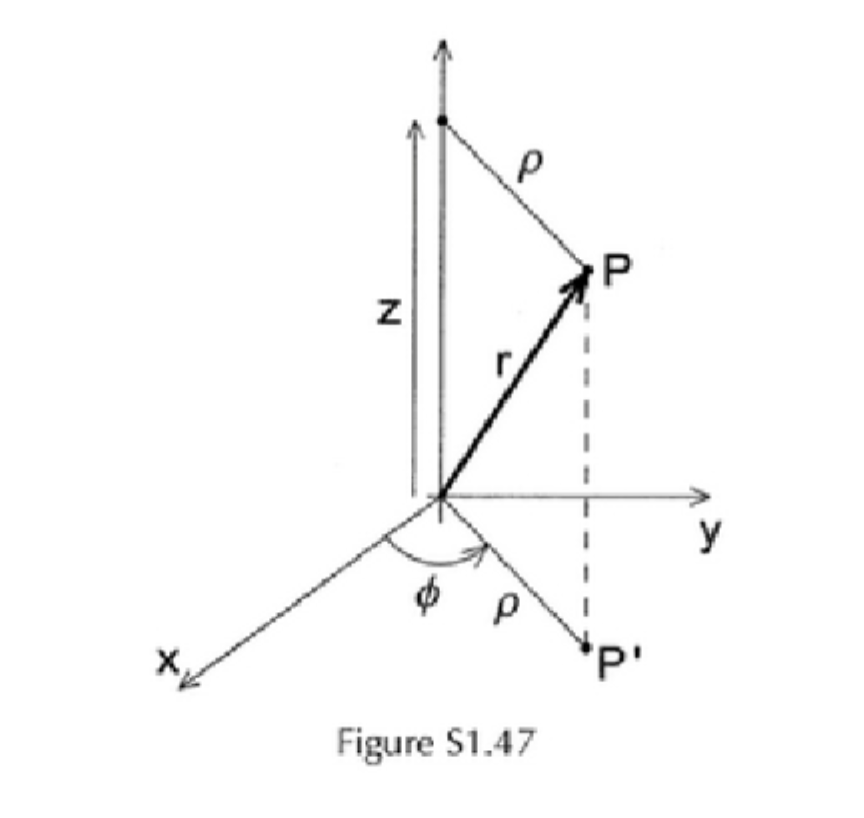
\includegraphics[width=0.5\textwidth]{coor.png}
    \label{coord}
    \caption{Sketch to illustrate the three cylindrical coordinates.}
\end{figure}
    

    \item \textbf{Expressions for $\rho, \phi, z$:}
    Based on the definitions from 2D polar coordinates applied to the $xy$-plane:
    \begin{itemize}
        \item From the Pythagorean theorem in the $xy$-plane:
        $$\rho = \sqrt{x^2 + y^2}$$
        \item From the trigonometry of the triangle $OP'x$:
        $$\phi = \arctan\left(\frac{y}{x}\right)$$
        (More precisely, $\phi = \operatorname{atan2}(y, x)$ to account for all quadrants).
        \item The $z$-coordinate is unchanged:
        $$z = z$$
    \end{itemize}

    \item \textbf{Explanation of $\rho$:}
    The coordinate $\rho$ is the \textbf{perpendicular distance of the point $P$ from the $z$-axis}.

    \item \textbf{The $r$ vs. $\rho$ Notation:}
    Using $r$ instead of $\rho$ for the cylindrical radial coordinate is \textbf{unfortunate} because in 3D problems, $r$ is almost universally reserved for the \textbf{spherical radial coordinate}:
    $$r = |\mathbf{r}| = \sqrt{x^2 + y^2 + z^2}$$
    This $r$ represents the distance from the point $P$ directly to the \textbf{origin}.
    
    If $r$ were used for the cylindrical coordinate ($\rho$), it would be ambiguous whether $r$ meant $\sqrt{x^2+y^2}$ or $\sqrt{x^2+y^2+z^2}$. Using $\rho$ avoids this confusion.
\end{enumerate}

\hrulefill

\subsection*{(b) Unit Vectors and Position Vector}

\begin{enumerate}
    \item \textbf{Description of Unit Vectors:}
    \begin{itemize}
        \item \textbf{$\hat{\rho}$:} The radial unit vector. It lies parallel to the $xy$-plane, points in the direction of increasing $\rho$, and is directed radially \textbf{outward from the $z$-axis}.
        \item \textbf{$\hat{\phi}$:} The tangential or azimuthal unit vector. It lies parallel to the $xy$-plane, points in the direction of increasing $\phi$, and is tangent to the circle of constant $\rho$ and $z$. It is perpendicular to $\hat{\rho}$ (i.e., $\hat{\rho} \cdot \hat{\phi} = 0$).
        \item \textbf{$\hat{\mathbf{z}}$:} The vertical unit vector. It points in the direction of increasing $z$ (parallel to the $z$-axis). It is identical to the Cartesian unit vector $\hat{\mathbf{k}}$.
    \end{itemize}

    \item \textbf{Expansion of the Position Vector $\mathbf{r}$:}
    The position vector $\mathbf{r}$ is the vector from the origin $O$ to the point $P$. We can write this vector as the sum of a vector from $O$ to $P'$ and a vector from $P'$ to $P$.
    \begin{itemize}
        \item The vector from $O$ to $P'$ is the 2D position vector in the $xy$-plane. In polar coordinates, this is simply $\rho \hat{\rho}$.
        \item The vector from $P'$ to $P$ is a vertical vector of length $z$, which is $z \hat{\mathbf{z}}$.
    \end{itemize}
    
    Combining these, the position vector $\mathbf{r}$ is:
    $$\mathbf{r} = \rho \hat{\rho} + z \hat{\mathbf{z}}$$
\end{enumerate}

\hrulefill

\subsection*{(c) Finding the Acceleration $\mathbf{a} = \ddot{\mathbf{r}}$}

To find the acceleration $\mathbf{a} = \ddot{\mathbf{r}}$, we must differentiate $\mathbf{r}$ twice with respect to time $t$.

\begin{enumerate}
    \item \textbf{Derivatives of Unit Vectors:}
    The unit vectors $\hat{\rho}$ and $\hat{\phi}$ are not constant; their directions change as the particle moves (specifically, as $\phi(t)$ changes). The unit vector $\hat{\mathbf{z}}$ is constant. Using the chain rule on their Cartesian definitions (or quoting the 2D results) gives:
    \begin{itemize}
        \item $\dot{\hat{\rho}} = \frac{d}{dt}(\cos\phi \hat{\mathbf{i}} + \sin\phi \hat{\mathbf{j}}) = (-\sin\phi \cdot \dot{\phi})\hat{\mathbf{i}} + (\cos\phi \cdot \dot{\phi})\hat{\mathbf{j}} = \dot{\phi}(-\sin\phi \hat{\mathbf{i}} + \cos\phi \hat{\mathbf{j}}) = \dot{\phi}\hat{\phi}$
        \item $\dot{\hat{\phi}} = \frac{d}{dt}(-\sin\phi \hat{\mathbf{i}} + \cos\phi \hat{\mathbf{j}}) = (-\cos\phi \cdot \dot{\phi})\hat{\mathbf{i}} + (-\sin\phi \cdot \dot{\phi})\hat{\mathbf{j}} = -\dot{\phi}(\cos\phi \hat{\mathbf{i}} + \sin\phi \hat{\mathbf{j}}) = -\dot{\phi}\hat{\rho}$
        \item $\dot{\hat{\mathbf{z}}} = \frac{d}{dt}(\hat{\mathbf{k}}) = 0$
    \end{itemize}

    Summary of derivatives:
    $$\dot{\hat{\rho}} = \dot{\phi} \hat{\phi}$$
    $$\dot{\hat{\phi}} = -\dot{\phi} \hat{\rho}$$
    $$\dot{\hat{\mathbf{z}}} = 0$$

    \item \textbf{First Derivative (Velocity $\mathbf{v}$):}
    We differentiate $\mathbf{r} = \rho \hat{\rho} + z \hat{\mathbf{z}}$ using the product rule:
    $$\mathbf{v} = \dot{\mathbf{r}} = \frac{d}{dt}(\rho \hat{\rho}) + \frac{d}{dt}(z \hat{\mathbf{z}})$$
    $$\mathbf{v} = (\dot{\rho} \hat{\rho} + \rho \dot{\hat{\rho}}) + (\dot{z} \hat{\mathbf{z}} + z \dot{\hat{\mathbf{z}}})$$
    
    Now substitute the unit vector derivatives:
    $$\mathbf{v} = (\dot{\rho} \hat{\rho} + \rho (\dot{\phi} \hat{\phi})) + (\dot{z} \hat{\mathbf{z}} + z (0))$$
    
    The velocity vector is:
    $$\mathbf{v} = \dot{\rho} \hat{\rho} + \rho \dot{\phi} \hat{\phi} + \dot{z} \hat{\mathbf{z}}$$

    \item \textbf{Second Derivative (Acceleration $\mathbf{a}$):}
    We differentiate the velocity vector $\mathbf{v}$ using the product rule for all three terms.
    $$\mathbf{a} = \dot{\mathbf{v}} = \frac{d}{dt}(\dot{\rho} \hat{\rho}) + \frac{d}{dt}(\rho \dot{\phi} \hat{\phi}) + \frac{d}{dt}(\dot{z} \hat{\mathbf{z}})$$

    \begin{itemize}
        \item \textbf{Term 1:} $\frac{d}{dt}(\dot{\rho} \hat{\rho}) = \ddot{\rho} \hat{\rho} + \dot{\rho} \dot{\hat{\rho}} = \ddot{\rho} \hat{\rho} + \dot{\rho}(\dot{\phi} \hat{\phi})$
        \item \textbf{Term 2:} $\frac{d}{dt}(\rho \dot{\phi} \hat{\phi}) = (\dot{\rho})(\dot{\phi} \hat{\phi}) + (\rho)(\ddot{\phi} \hat{\phi}) + (\rho \dot{\phi})(\dot{\hat{\phi}})$
        $$= \dot{\rho} \dot{\phi} \hat{\phi} + \rho \ddot{\phi} \hat{\phi} + \rho \dot{\phi}(-\dot{\phi} \hat{\rho})$$
        $$= \dot{\rho} \dot{\phi} \hat{\phi} + \rho \ddot{\phi} \hat{\phi} - \rho \dot{\phi}^2 \hat{\rho}$$
        \item \textbf{Term 3:} $\frac{d}{dt}(\dot{z} \hat{\mathbf{z}}) = \ddot{z} \hat{\mathbf{z}} + \dot{z} \dot{\hat{\mathbf{z}}} = \ddot{z} \hat{\mathbf{z}} + \dot{z}(0) = \ddot{z} \hat{\mathbf{z}}$
    \end{itemize}

    \item \textbf{Assemble and Group:}
    Now we add all the pieces of $\mathbf{a}$ back together:
    $$\mathbf{a} = \left( \ddot{\rho} \hat{\rho} + \dot{\rho} \dot{\phi} \hat{\phi} \right) + \left( \dot{\rho} \dot{\phi} \hat{\phi} + \rho \ddot{\phi} \hat{\phi} - \rho \dot{\phi}^2 \hat{\rho} \right) + \left( \ddot{z} \hat{\mathbf{z}} \right)$$
    
    Finally, we group the terms by their unit vectors ($\hat{\rho}$, $\hat{\phi}$, $\hat{\mathbf{z}}$):
    \begin{itemize}
        \item \textbf{$\hat{\rho}$ terms:} $\ddot{\rho} \hat{\rho} - \rho \dot{\phi}^2 \hat{\rho} = (\ddot{\rho} - \rho \dot{\phi}^2) \hat{\rho}$
        \item \textbf{$\hat{\phi}$ terms:} $\dot{\rho} \dot{\phi} \hat{\phi} + \dot{\rho} \dot{\phi} \hat{\phi} + \rho \ddot{\phi} \hat{\phi} = (2 \dot{\rho} \dot{\phi} + \rho \ddot{\phi}) \hat{\phi}$
        \item \textbf{$\hat{\mathbf{z}}$ terms:} $\ddot{z} \hat{\mathbf{z}}$
    \end{itemize}

    The final expression for the acceleration vector is:
    $$\mathbf{a} = (\ddot{\rho} - \rho \dot{\phi}^2) \hat{\rho} + (2 \dot{\rho} \dot{\phi} + \rho \ddot{\phi}) \hat{\phi} + \ddot{z} \hat{\mathbf{z}}$$
    
    The cylindrical components of the acceleration are:
    \begin{itemize}
        \item $a_{\rho} = \ddot{\rho} - \rho \dot{\phi}^2$
        \item $a_{\phi} = 2 \dot{\rho} \dot{\phi} + \rho \ddot{\phi}$
        \item $a_z = \ddot{z}$
    \end{itemize}
\end{enumerate}

\newpage
\subsection*{4.2}

Evaluate the work done

\begin{equation}
    W = \int_0^P \mathbf{F} d\mathbf{r} = \int_0^P (F_x dx + F_y dy)
    \label{4.100}
\end{equation}

by the two-dimensional force $\mathbf{F}=(x^2, 2xy)$ along the three paths joining the origin to the point P = (1, 1) as shown in Fig.~\ref{fig:work} (\textbf{a}) and defined as follows: (\textbf{a}) This path goes along the x axis to Q = (1, 0) and then straight up to $P$. (Divide the integral into two pieces, $\int_O^P = \int_O^Q + \int_Q^P$.) (\textbf{b}) On this path $y=x^2$, and you can replace the term $dy$ in \ref{4.100}
by $dy=2x~dx$ and convert the whole integral into an integral over $x$. (\textbf{c}) This path is given parametrically as $x=t^3$, $y=t^2$. In this case rewrite $x, y, dx,$ and $dy$ in equation \ref{4.100} in terms of $t$ and $dt$, and convert the integral into an integral over $t$.

\begin{figure}[h]
	\begin{center}
		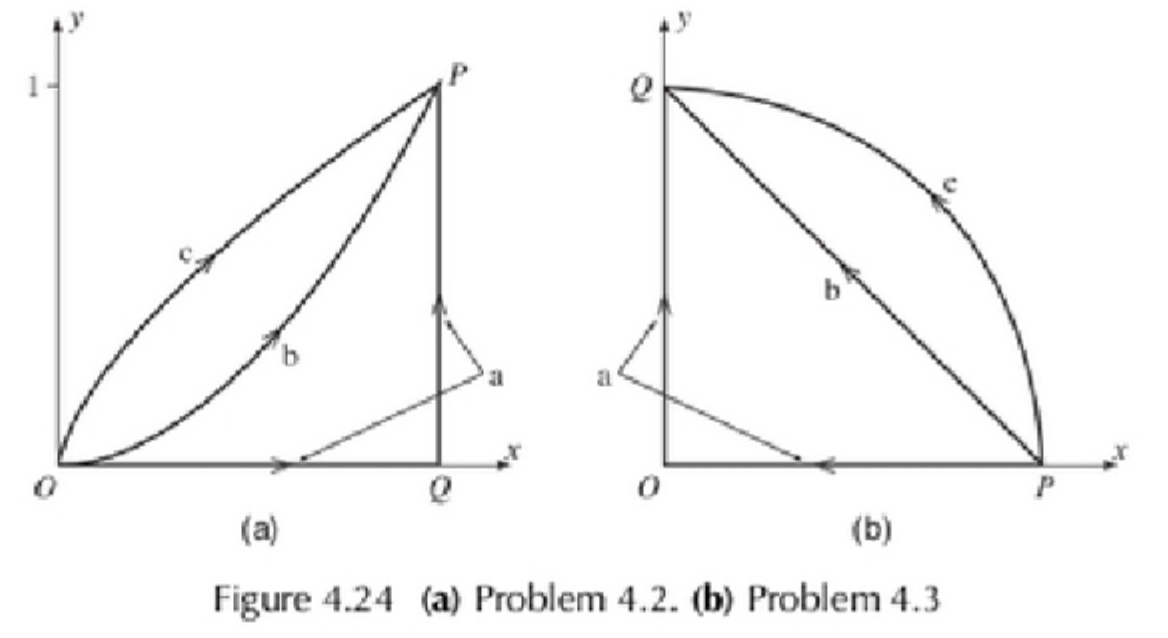
\includegraphics[width=0.5\textwidth]{4.24.png}
	\end{center}
	\caption{(\textbf{a}) Problem 4.2. (\textbf{b}) Problem 4.3} 
 \label{fig:work}
\end{figure}

\textbf{Answer}:

The force is $\mathbf{F} = (x^2, 2xy)$, and the work integral is:
$$W = \int_O^P (F_x dx + F_y dy) = \int_{(0,0)}^{(1,1)} (x^2 dx + 2xy dy)$$

\hrulefill

\section*{(a) Path O $\to$ Q $\to$ P}

This path is broken into two straight-line segments. We will calculate the work for each segment and add them.
$$W_a = W_{OQ} + W_{QP}$$

\textbf{1. Path O $\to$ Q:}
\begin{itemize}
    \item \textbf{Path:} From $O=(0,0)$ to $Q=(1,0)$.
    \item \textbf{Constraints:} Along this segment, $y=0$.
    \item \textbf{Differential:} Because $y$ is constant, its differential $dy = 0$.
    \item \textbf{Integration:} We substitute $y=0$ and $dy=0$ into the work integral. The integral is with respect to $x$, which goes from $0$ to $1$.
    $$W_{OQ} = \int_{x=0}^{x=1} (x^2 dx + 2x(0)(0)) = \int_0^1 x^2 dx$$
    \item \textbf{Evaluation:}
    $$W_{OQ} = \left[ \frac{1}{3}x^3 \right]_0^1 = \frac{1}{3}(1)^3 - \frac{1}{3}(0)^3 = \frac{1}{3}$$
\end{itemize}

\textbf{2. Path Q $\to$ P:}
\begin{itemize}
    \item \textbf{Path:} From $Q=(1,0)$ to $P=(1,1)$.
    \item \textbf{Constraints:} Along this segment, $x=1$.
    \item \textbf{Differential:} Because $x$ is constant, its differential $dx = 0$.
    \item \textbf{Integration:} We substitute $x=1$ and $dx=0$ into the work integral. The integral is with respect to $y$, which goes from $0$ to $1$.
    $$W_{QP} = \int_{y=0}^{y=1} ((1)^2(0) + 2(1)y dy) = \int_0^1 2y dy$$
    \item \textbf{Evaluation:}
    $$W_{QP} = \left[ y^2 \right]_0^1 = (1)^2 - (0)^2 = 1$$
\end{itemize}

\textbf{3. Total Work $W_a$:}
\begin{itemize}
    \item $$W_a = W_{OQ} + W_{QP} = \frac{1}{3} + 1 = \frac{4}{3}$$
\end{itemize}

\hrulefill

\section*{(b) Path $y = x^2$}

\begin{itemize}
    \item \textbf{Path:} A parabolic path from $O=(0,0)$ to $P=(1,1)$.
    \item \textbf{Constraints:} We are given $y = x^2$.
    \item \textbf{Differential:} Differentiating the constraint gives $dy = 2x dx$.
    \item \textbf{Integration:} We substitute $y=x^2$ and $dy=2x dx$ into the work integral. This converts the entire integral into terms of $x$, which goes from $0$ to $1$.
    $$W_b = \int_{x=0}^{x=1} (x^2 dx + 2x(y) dy)$$
    $$W_b = \int_0^1 \left( x^2 dx + 2x(x^2) (2x dx) \right)$$
    $$W_b = \int_0^1 \left( x^2 dx + 4x^4 dx \right) = \int_0^1 (x^2 + 4x^4) dx$$
    \item \textbf{Evaluation:}
    $$W_b = \left[ \frac{1}{3}x^3 + \frac{4}{5}x^5 \right]_0^1$$
    $$W_b = \left( \frac{1}{3}(1)^3 + \frac{4}{5}(1)^5 \right) - (0) = \frac{1}{3} + \frac{4}{5}$$
    $$W_b = \frac{5}{15} + \frac{12}{15} = \frac{17}{15}$$
\end{itemize}

\hrulefill

\section*{(c) Path $x = t^3, y = t^2$}

\begin{itemize}
    \item \textbf{Path:} A parametric path. We must find the limits for $t$.
    \begin{itemize}
        \item At the origin $O=(0,0)$: $x=0=t^3$ and $y=0=t^2$. This gives $t=0$.
        \item At the point $P=(1,1)$: $x=1=t^3$ and $y=1=t^2$. This gives $t=1$.
        \item The path is traced as $t$ goes from $0$ to $1$.
    \end{itemize}
    \item \textbf{Constraints:}
    \begin{itemize}
        \item $x = t^3$
        \item $y = t^2$
    \end{itemize}
    \item \textbf{Differentials:}
    \begin{itemize}
        \item $dx = 3t^2 dt$
        \item $dy = 2t dt$
    \end{itemize}
    \item \textbf{Integration:} We substitute $x, y, dx,$ and $dy$ into the work integral to get an integral in $t$.
    $$W_c = \int_{t=0}^{t=1} (x^2 dx + 2xy dy)$$
    $$W_c = \int_0^1 \left( (t^3)^2 (3t^2 dt) + 2(t^3)(t^2) (2t dt) \right)$$
    $$W_c = \int_0^1 \left( (t^6)(3t^2) + (2t^5)(2t) \right) dt$$
    $$W_c = \int_0^1 (3t^8 + 4t^6) dt$$
    \item \textbf{Evaluation:}
    $$W_c = \left[ \frac{3}{9}t^9 + \frac{4}{7}t^7 \right]_0^1 = \left[ \frac{1}{3}t^9 + \frac{4}{7}t^7 \right]_0^1$$
    $$W_c = \left( \frac{1}{3}(1)^9 + \frac{4}{7}(1)^7 \right) - (0) = \frac{1}{3} + \frac{4}{7}$$
    $$W_c = \frac{7}{21} + \frac{12}{21} = \frac{19}{21}$$
\end{itemize}

\newpage
\subsection*{4.3}

Do the same as Problem 4.2, but for the force $\mathbf{F} = (-y, x)$ and for the three paths joining $P$ and $Q$ shown in Fig.~\ref{fig:work}(b) and defined as follows: (\textbf{a}) This path goes straight from $P = (1, 0)$ to the origin and then straight to $Q = (0,1)$. (\textbf{b}) This is a straight line from $P$ to $Q$. (Write $y$ as a function of $x$ and rewrite the integral as an integral over $x$.) (\textbf{c}) This is a quarter-circle centered on the origin. (Write $x$ and $y$ in polar coordinates and rewrite the integral as an integral over $\phi$.)

\textbf{Answer}:

The force is $\mathbf{F} = (F_x, F_y) = (-y, x)$. We need to evaluate the work done, $W$, from the starting point $P = (1, 0)$ to the end point $Q = (0, 1)$ along three different paths.

The work integral is:
$$W = \int_P^Q \mathbf{F} \cdot d\mathbf{r} = \int_{(1,0)}^{(0,1)} (F_x dx + F_y dy) = \int_{(1,0)}^{(0,1)} (-y dx + x dy)$$

\hrulefill

\section*{(a) Path $P \to O \to Q$}

This path consists of two straight-line segments: from $P=(1,0)$ to the origin $O=(0,0)$, and then from $O=(0,0)$ to $Q=(0,1)$. We calculate the work for each segment and add them.
$$W_a = W_{PO} + W_{OQ}$$

\textbf{1. Path $P \to O$:}
\begin{itemize}
    \item \textbf{Path:} From $P=(1,0)$ to $O=(0,0)$.
    \item \textbf{Constraints:} The path is along the $x$-axis, so $y=0$.
    \item \textbf{Differential:} Since $y$ is constant, $dy = 0$.
    \item \textbf{Integration:} We substitute $y=0$ and $dy=0$ into the work integral. The integral is with respect to $x$, which goes from $1$ to $0$.
    $$W_{PO} = \int_{x=1}^{x=0} (-y dx + x dy) = \int_1^0 (-(0) dx + x(0)) = \int_1^0 0 dx$$
    \item \textbf{Evaluation:}
    $$W_{PO} = 0$$
\end{itemize}

\textbf{2. Path $O \to Q$:}
\begin{itemize}
    \item \textbf{Path:} From $O=(0,0)$ to $Q=(0,1)$.
    \item \textbf{Constraints:} The path is along the $y$-axis, so $x=0$.
    \item \textbf{Differential:} Since $x$ is constant, $dx = 0$.
    \item \textbf{Integration:} We substitute $x=0$ and $dx=0$ into the work integral. The integral is with respect to $y$, which goes from $0$ to $1$.
    $$W_{OQ} = \int_{y=0}^{y=1} (-y dx + x dy) = \int_0^1 (-y(0) + (0)dy) = \int_0^1 0 dy$$
    \item \textbf{Evaluation:}
    $$W_{OQ} = 0$$
\end{itemize}

\textbf{3. Total Work $W_a$:}
\begin{itemize}
    \item $$W_a = W_{PO} + W_{OQ} = 0 + 0 = 0$$
\end{itemize}

\hrulefill

\section*{(b) Straight Line from $P$ to $Q$}

\begin{itemize}
    \item \textbf{Path:} A straight line from $P=(1,0)$ to $Q=(0,1)$.
    \item \textbf{Constraints:} We find the equation of the line, $y = mx + b$.
    \begin{itemize}
        \item The slope $m = \frac{\Delta y}{\Delta x} = \frac{1-0}{0-1} = -1$.
        \item The $y$-intercept is at $Q=(0,1)$, so $b=1$.
        \item The equation of the path is $y = -x + 1$.
    \end{itemize}
    \item \textbf{Differential:} Differentiating the constraint gives $dy = -dx$.
    \item \textbf{Integration:} We substitute $y = -x + 1$ and $dy = -dx$ into the work integral. This converts the entire integral into terms of $x$. The path starts at $x=1$ (point $P$) and ends at $x=0$ (point $Q$).
    $$W_b = \int_{x=1}^{x=0} (-y dx + x dy)$$
    $$W_b = \int_1^0 \left( -(-x+1) dx + x(-dx) \right)$$
    $$W_b = \int_1^0 \left( (x-1) dx - x dx \right)$$
    $$W_b = \int_1^0 (x - 1 - x) dx = \int_1^0 (-1) dx$$
    \item \textbf{Evaluation:}
    $$W_b = \left[ -x \right]_1^0 = (-0) - (-1) = 1$$
\end{itemize}

\hrulefill

\section*{(c) Quarter-Circle Path}

\begin{itemize}
    \item \textbf{Path:} A quarter-circle of radius $R=1$, centered at the origin. The path starts at $P=(1,0)$ and ends at $Q=(0,1)$.
    \item \textbf{Constraints (Polar Coordinates):}
    \begin{itemize}
        \item $x = R \cos\phi = 1 \cos\phi = \cos\phi$
        \item $y = R \sin\phi = 1 \sin\phi = \sin\phi$
        \item The path starts at $\phi = 0$ (point $P$) and ends at $\phi = \pi/2$ (point $Q$).
    \end{itemize}
    \item \textbf{Differentials:}
    \begin{itemize}
        \item $dx = -\sin\phi d\phi$
        \item $dy = \cos\phi d\phi$
    \end{itemize}
    \item \textbf{Integration:} We substitute $x, y, dx,$ and $dy$ into the work integral to get an integral in terms of $\phi$, which runs from $0$ to $\pi/2$.
    $$W_c = \int_{\phi=0}^{\phi=\pi/2} (-y dx + x dy)$$
    $$W_c = \int_0^{\pi/2} \left( -(\sin\phi) (-\sin\phi d\phi) + (\cos\phi) (\cos\phi d\phi) \right)$$
    $$W_c = \int_0^{\pi/2} \left( \sin^2\phi d\phi + \cos^2\phi d\phi \right)$$
    Using the identity $\sin^2\phi + \cos^2\phi = 1$:
    $$W_c = \int_0^{\pi/2} (1) d\phi$$
    \item \textbf{Evaluation:}
    $$W_c = \left[ \phi \right]_0^{\pi/2} = \frac{\pi}{2} - 0 = \frac{\pi}{2}$$
\end{itemize}

\newpage
\subsection*{4.21}

Verify that the gravitational force $-GMn\hat{\mathbf{r}}/r^2$ on a point mass $m$ at $\mathbf{r}$, due to a fixed point mass M at the origin, is conservative and calculate the corresponding potential energy.

\textbf{Answer}:

\section*{Part 1: Verifying the Force is Conservative}

A force $\mathbf{F}$ is defined as \textbf{conservative} if its curl is zero: $\nabla \times \mathbf{F} = \mathbf{0}$.

\begin{enumerate}
    \item \textbf{Express the Force in Spherical Coordinates:}
    The gravitational force $\mathbf{F} = -GMm\hat{\mathbf{r}}/r^2$ is a central force, meaning it only has a radial component. In spherical polar coordinates, we can write the force vector as:
    $$\mathbf{F} = F_r \hat{\mathbf{r}} + F_\theta \hat{\mathbf{\theta}} + F_\phi \hat{\mathbf{\phi}}$$
    Comparing this to the given force, we have:
    \begin{itemize}
        \item $F_r = -\frac{GMm}{r^2}$
        \item $F_\theta = 0$
        \item $F_\phi = 0$
    \end{itemize}

    \item \textbf{Write the Curl in Spherical Coordinates:}
    The formula for the curl ($\nabla \times \mathbf{F}$) in spherical coordinates is:
\begin{align*}
\nabla \times \mathbf{F} = & \frac{1}{r^2 \sin\theta} \left[ \frac{\partial}{\partial \theta}(r \sin\theta F_\phi) - \frac{\partial}{\partial \phi}(r F_\theta) \right] \hat{\mathbf{r}} \\
& + \frac{1}{r \sin\theta} \left[ \frac{\partial}{\partial \phi}(F_r) - \frac{\partial}{\partial r}(r \sin\theta F_\phi) \right] \hat{\mathbf{\theta}} \\
& + \frac{1}{r} \left[ \frac{\partial}{\partial r}(r F_\theta) - \frac{\partial}{\partial \theta}(F_r) \right] \hat{\mathbf{\phi}}
\end{align*}

    \item \textbf{Evaluate Each Component of the Curl:}
    We substitute our components $F_r$, $F_\theta$, and $F_\phi$ into this formula.

    \begin{itemize}
        \item \textbf{$\hat{\mathbf{r}}$ component:}
        $$\frac{1}{r^2 \sin\theta} \left[ \frac{\partial}{\partial \theta}(r \sin\theta \cdot 0) - \frac{\partial}{\partial \phi}(r \cdot 0) \right] = \frac{1}{r^2 \sin\theta} [0 - 0] = 0$$

        \item \textbf{$\hat{\mathbf{\theta}}$ component:}
        Here we must evaluate $\frac{\partial}{\partial \phi}(F_r)$. Since $F_r = -GMm/r^2$ does not depend on $\phi$, this partial derivative is zero.
        $$\frac{1}{r \sin\theta} \left[ \frac{\partial}{\partial \phi}\left(-\frac{GMm}{r^2}\right) - \frac{\partial}{\partial r}(r \sin\theta \cdot 0) \right] = \frac{1}{r \sin\theta} [0 - 0] = 0$$

        \item \textbf{$\hat{\mathbf{\phi}}$ component:}
        Here we must evaluate $\frac{\partial}{\partial \theta}(F_r)$. Since $F_r = -GMm/r^2$ does not depend on $\theta$, this partial derivative is also zero.
        $$\frac{1}{r} \left[ \frac{\partial}{\partial r}(r \cdot 0) - \frac{\partial}{\partial \theta}\left(-\frac{GMm}{r^2}\right) \right] = \frac{1}{r} [0 - 0] = 0$$
    \end{itemize}

    \item \textbf{Conclusion:}
    Since all three components of the curl are zero, we have $\nabla \times \mathbf{F} = \mathbf{0}$. This verifies that the gravitational force is \textbf{conservative}.
\end{enumerate}

\hrulefill

\section*{Part 2: Calculating the Potential Energy}

\begin{enumerate}
    \item \textbf{Definition of Potential Energy:}
    The potential energy $U$ is defined by the relation $\mathbf{F} = -\nabla U$. We can find $U$ by integrating this expression. The change in potential energy when moving from a reference point $\mathbf{r}_{\text{ref}}$ to a point $\mathbf{r}$ is:
    $$U(\mathbf{r}) - U(\mathbf{r}_{\text{ref}}) = - \int_{\mathbf{r}_{\text{ref}}}^{\mathbf{r}} \mathbf{F} \cdot d\mathbf{r}$$

    \item \textbf{Set the Reference Point:}
    By convention, the reference point for gravitational potential energy is taken at infinity ($\mathbf{r}_{\text{ref}} = \infty$), where the potential energy is defined to be zero ($U(\infty) = 0$).
    $$U(\mathbf{r}) - U(\infty) = - \int_{\infty}^{\mathbf{r}} \mathbf{F} \cdot d\mathbf{r}$$
    $$U(\mathbf{r}) = - \int_{\infty}^{\mathbf{r}} \mathbf{F} \cdot d\mathbf{r}$$

    \item \textbf{Set up the Integral:}
    Because the force is conservative, the integral is path-independent. We can choose the simplest possible path: a straight radial line from $r' = \infty$ to $r' = r$.
    \begin{itemize}
        \item The force is $\mathbf{F} = -\frac{GMm}{r'^2}\hat{\mathbf{r}}$. (We use $r'$ as the integration variable).
        \item The path differential $d\mathbf{r}$ along this radial path is $d\mathbf{r} = dr' \hat{\mathbf{r}}$.
    \end{itemize}

    \item \textbf{Evaluate the Integral:}
    We substitute these into the integral:
    $$U(r) = - \int_{\infty}^{r} \left( -\frac{GMm}{r'^2}\hat{\mathbf{r}} \right) \cdot (dr' \hat{\mathbf{r}})$$
    
    The dot product $\hat{\mathbf{r}} \cdot \hat{\mathbf{r}} = 1$, which simplifies the integral:
    $$U(r) = - \int_{\infty}^{r} \left( -\frac{GMm}{r'^2} \right) dr'$$
    $$U(r) = GMm \int_{\infty}^{r} r'^{-2} dr'$$
    
    Now, we perform the integration:
    $$U(r) = GMm \left[ \frac{r'^{-1}}{-1} \right]_{\infty}^{r} = GMm \left[ -\frac{1}{r'} \right]_{\infty}^{r}$$
    
    Finally, we evaluate the definite integral at its limits:
    $$U(r) = GMm \left( \left( -\frac{1}{r} \right) - \left( -\frac{1}{\infty} \right) \right)$$
    
    The term $1/\infty$ goes to $0$.

    \item \textbf{Final Result:}
    The potential energy corresponding to the gravitational force is:
    $$U(r) = -\frac{GMm}{r}$$
\end{enumerate}

\newpage
\subsection*{4.23}

Which of the following forces is conservative? (\textbf{a}) $\mathbf{F} = k(x, 2y, 3z)$ where $k$ is a constant.(\textbf{b}) $\mathbf{F} = k(x,y,0)$. (\textbf{c}) $\mathbf{F} = k(-y,x,0)$. For those which are conservative, find the corresponding potential energy $U$, and verify by direct differentiation that $\mathbf{F} = - \nabla U$.

\textbf{Answer}:

A force $\mathbf{F}$ is \textbf{conservative} if its curl is zero, i.e., $\nabla \times \mathbf{F} = 0$. The curl is calculated as:
$$ \nabla \times \mathbf{F} = \begin{vmatrix}
\hat{\mathbf{x}} & \hat{\mathbf{y}} & \hat{\mathbf{z}} \\
\frac{\partial}{\partial x} & \frac{\partial}{\partial y} & \frac{\partial}{\partial z} \\
F_x & F_y & F_z
\end{vmatrix} = \left( \frac{\partial F_z}{\partial y} - \frac{\partial F_y}{\partial z} \right) \hat{\mathbf{x}} + \left( \frac{\partial F_x}{\partial z} - \frac{\partial F_z}{\partial x} \right) \hat{\mathbf{y}} + \left( \frac{\partial F_y}{\partial x} - \frac{\partial F_x}{\partial y} \right) \hat{\mathbf{z}} $$

If a force is conservative, its potential energy $U$ can be found by integrating the relation $\mathbf{F} = -\nabla U$, which means:
\begin{itemize}
    \item $F_x = -\frac{\partial U}{\partial x}$
    \item $F_y = -\frac{\partial U}{\partial y}$
    \item $F_z = -\frac{\partial U}{\partial z}$
\end{itemize}

\hrulefill

\section*{(a) $\mathbf{F} = k(x, 2y, 3z)$}

Here, $F_x = kx$, $F_y = 2ky$, and $F_z = 3kz$.

\subsection*{Step 1: Check if the force is conservative}
We calculate the curl of $\mathbf{F}$:
\begin{itemize}
    \item $\hat{\mathbf{x}}$ component: $\frac{\partial F_z}{\partial y} - \frac{\partial F_y}{\partial z} = \frac{\partial}{\partial y}(3kz) - \frac{\partial}{\partial z}(2ky) = 0 - 0 = 0$
    \item $\hat{\mathbf{y}}$ component: $\frac{\partial F_x}{\partial z} - \frac{\partial F_z}{\partial x} = \frac{\partial}{\partial z}(kx) - \frac{\partial}{\partial x}(3kz) = 0 - 0 = 0$
    \item $\hat{\mathbf{z}}$ component: $\frac{\partial F_y}{\partial x} - \frac{\partial F_x}{\partial y} = \frac{\partial}{\partial x}(2ky) - \frac{\partial}{\partial y}(kx) = 0 - 0 = 0$
\end{itemize}
Since $\nabla \times \mathbf{F} = 0$, \textbf{force (a) is conservative.}

\subsection*{Step 2: Find the potential energy $U$}
We integrate the components of $\mathbf{F} = -\nabla U$:
\begin{enumerate}
    \item $F_x = -\frac{\partial U}{\partial x} \implies kx = -\frac{\partial U}{\partial x}$ \\
    Integrating with respect to $x$:
    $U = -\int kx \, dx = -\frac{1}{2}kx^2 + g(y, z)$ (where $g(y, z)$ is an integration constant with respect to $x$).

    \item $F_y = -\frac{\partial U}{\partial y} \implies 2ky = -\frac{\partial}{\partial y}\left(-\frac{1}{2}kx^2 + g(y, z)\right) = -\frac{\partial g}{\partial y}$ \\
    Integrating $\frac{\partial g}{\partial y} = -2ky$ with respect to $y$:
    $g(y, z) = -\int 2ky \, dy = -ky^2 + h(z)$ (where $h(z)$ is an integration constant with respect to $y$). \\
    \emph{So far, $U = -\frac{1}{2}kx^2 - ky^2 + h(z)$.}

    \item $F_z = -\frac{\partial U}{\partial z} \implies 3kz = -\frac{\partial}{\partial z}\left(-\frac{1}{2}kx^2 - ky^2 + h(z)\right) = -\frac{dh}{dz}$ \\
    Integrating $\frac{dh}{dz} = -3kz$ with respect to $z$:
    $h(z) = -\int 3kz \, dz = -\frac{3}{2}kz^2 + C$ (where $C$ is a constant).
\end{enumerate}
Setting the integration constant $C=0$, the potential energy is:
$$\boldsymbol{U(x, y, z) = -k\left(\frac{1}{2}x^2 + y^2 + \frac{3}{2}z^2\right)}$$

\subsection*{Step 3: Verify $\mathbf{F} = -\nabla U$}
$$-\nabla U = -\left(\frac{\partial U}{\partial x}\hat{\mathbf{x}} + \frac{\partial U}{\partial y}\hat{\mathbf{y}} + \frac{\partial U}{\partial z}\hat{\mathbf{z}}\right)$$
\begin{itemize}
    \item $-\frac{\partial U}{\partial x} = -\frac{\partial}{\partial x}\left(-\frac{1}{2}kx^2\right) = -(-kx) = kx$
    \item $-\frac{\partial U}{\partial y} = -\frac{\partial}{\partial y}\left(-ky^2\right) = -(-2ky) = 2ky$
    \item $-\frac{\partial U}{\partial z} = -\frac{\partial}{\partial z}\left(-\frac{3}{2}kz^2\right) = -(-3kz) = 3kz$
\end{itemize}
Thus, $-\nabla U = (kx, 2ky, 3kz) = \mathbf{F}$. \textbf{The verification is successful.}

\hrulefill

\section*{(b) $\mathbf{F} = k(x, y, 0)$}

Here, $F_x = kx$, $F_y = ky$, and $F_z = 0$.

\subsection*{Step 1: Check if the force is conservative}
We calculate the curl of $\mathbf{F}$:
\begin{itemize}
    \item $\hat{\mathbf{x}}$ component: $\frac{\partial F_z}{\partial y} - \frac{\partial F_y}{\partial z} = \frac{\partial}{\partial y}(0) - \frac{\partial}{\partial z}(ky) = 0 - 0 = 0$
    \item $\hat{\mathbf{y}}$ component: $\frac{\partial F_x}{\partial z} - \frac{\partial F_z}{\partial x} = \frac{\partial}{\partial z}(kx) - \frac{\partial}{\partial x}(0) = 0 - 0 = 0$
    \item $\hat{\mathbf{z}}$ component: $\frac{\partial F_y}{\partial x} - \frac{\partial F_x}{\partial y} = \frac{\partial}{\partial x}(ky) - \frac{\partial}{\partial y}(kx) = 0 - 0 = 0$
\end{itemize}
Since $\nabla \times \mathbf{F} = 0$, \textbf{force (b) is conservative.}

\subsection*{Step 2: Find the potential energy $U$}
We integrate the components of $\mathbf{F} = -\nabla U$:
\begin{enumerate}
    \item $F_x = -\frac{\partial U}{\partial x} \implies kx = -\frac{\partial U}{\partial x}$ \\
    Integrating with respect to $x$:
    $U = -\int kx \, dx = -\frac{1}{2}kx^2 + g(y, z)$

    \item $F_y = -\frac{\partial U}{\partial y} \implies ky = -\frac{\partial}{\partial y}\left(-\frac{1}{2}kx^2 + g(y, z)\right) = -\frac{\partial g}{\partial y}$ \\
    Integrating $\frac{\partial g}{\partial y} = -ky$ with respect to $y$:
    $g(y, z) = -\int ky \, dy = -\frac{1}{2}ky^2 + h(z)$ \\
    \emph{So far, $U = -\frac{1}{2}kx^2 - \frac{1}{2}ky^2 + h(z)$.}

    \item $F_z = -\frac{\partial U}{\partial z} \implies 0 = -\frac{\partial}{\partial z}\left(-\frac{1}{2}kx^2 - \frac{1}{2}ky^2 + h(z)\right) = -\frac{dh}{dz}$ \\
    Integrating $\frac{dh}{dz} = 0$ with respect to $z$:
    $h(z) = C$ (where $C$ is a constant).
\end{enumerate}
Setting the integration constant $C=0$, the potential energy is:
$$\boldsymbol{U(x, y, z) = -\frac{k}{2}(x^2 + y^2)}$$

\subsection*{Step 3: Verify $\mathbf{F} = -\nabla U$}
$$-\nabla U = -\left(\frac{\partial U}{\partial x}\hat{\mathbf{x}} + \frac{\partial U}{\partial y}\hat{\mathbf{y}} + \frac{\partial U}{\partial z}\hat{\mathbf{z}}\right)$$
\begin{itemize}
    \item $-\frac{\partial U}{\partial x} = -\frac{\partial}{\partial x}\left(-\frac{1}{2}kx^2\right) = -(-kx) = kx$
    \item $-\frac{\partial U}{\partial y} = -\frac{\partial}{\partial y}\left(-\frac{1}{2}ky^2\right) = -(-ky) = ky$
    \item $-\frac{\partial U}{\partial z} = -\frac{\partial}{\partial z}\left( \text{constant w.r.t z} \right) = 0$
\end{itemize}
Thus, $-\nabla U = (kx, ky, 0) = \mathbf{F}$. \textbf{The verification is successful.}

\hrulefill

\section*{(c) $\mathbf{F} = k(-y, x, 0)$}

Here, $F_x = -ky$, $F_y = kx$, and $F_z = 0$.

\subsection*{Step 1: Check if the force is conservative}
We calculate the curl of $\mathbf{F}$:
\begin{itemize}
    \item $\hat{\mathbf{x}}$ component: $\frac{\partial F_z}{\partial y} - \frac{\partial F_y}{\partial z} = \frac{\partial}{\partial y}(0) - \frac{\partial}{\partial z}(kx) = 0 - 0 = 0$
    \item $\hat{\mathbf{y}}$ component: $\frac{\partial F_x}{\partial z} - \frac{\partial F_z}{\partial x} = \frac{\partial}{\partial z}(-ky) - \frac{\partial}{\partial x}(0) = 0 - 0 = 0$
    \item $\hat{\mathbf{z}}$ component: $\frac{\partial F_y}{\partial x} - \frac{\partial F_x}{\partial y} = \frac{\partial}{\partial x}(kx) - \frac{\partial}{\partial y}(-ky) = k - (-k) = 2k$
\end{itemize}
Since $\nabla \times \mathbf{F} = (0, 0, 2k) \neq 0$ (assuming $k \neq 0$), \textbf{force (c) is not conservative.} \\
(This force, which points tangentially around the $z$-axis, is a classic example of a non-conservative force. It does work on a particle moving in a circle in the $xy$-plane.)

\hrulefill

\section*{Summary}
\begin{itemize}
    \item \textbf{(a) $\mathbf{F} = k(x, 2y, 3z)$ is conservative.} $U = -k(\frac{1}{2}x^2 + y^2 + \frac{3}{2}z^2)$.
    \item \textbf{(b) $\mathbf{F} = k(x, y, 0)$ is conservative.} $U = -\frac{k}{2}(x^2 + y^2)$.
    \item \textbf{(c) $\mathbf{F} = k(-y, x, 0)$ is not conservative.}
\end{itemize}

\newpage
\subsection*{4.27}

Suppose that the force $\mathbf{F} (\mathbf{r}, t)$ depends on the time $t$ but still satisfies $\nabla \times \mathbf{F} = 0$. It is a mathematical fact (related to Stokes's theorem as discussed in Problem 4.25) that the work integral $\int_1^2 \mathbf{F} (\mathbf{r}, t) \cdot d \mathbf{r}$ (evaluated at any one time $t$) is independent of the path taken between the points 1 and 2. Use this to show that the time-dependent PE defined by equation (4.48) (which is $U(\mathbf{r}, t) = - \int_{r_0}^r \mathbf{F} (\mathbf{r}', t) \cdot d \mathbf{r}'$), for any fixed time $t$, has the claimed property that $\mathbf{F} (\mathbf{r}, t) = - \nabla U(\mathbf{r}, t)$. Can you see what goes wrong with the argument leading to Equation (4.19) (which is $\Delta (T + U) = 0$), that is conservation of energy?

\textbf{Answer}:

\section*{Part 1: Showing $\mathbf{F}(\mathbf{r}, t) = - \nabla U(\mathbf{r}, t)$}

Our goal is to show that the force $\mathbf{F}$ is the negative gradient of the potential energy $U$, given the definition:
$$U(\mathbf{r}, t) = - \int_{\mathbf{r}_0}^{\mathbf{r}} \mathbf{F}(\mathbf{r}', t) \cdot d\mathbf{r}'$$
Here, the time $t$ is held constant during the spatial integral.

The gradient in Cartesian coordinates is $\nabla U = \frac{\partial U}{\partial x}\hat{\mathbf{i}} + \frac{\partial U}{\partial y}\hat{\mathbf{j}} + \frac{\partial U}{\partial z}\hat{\mathbf{k}}$. Let's show that $F_x = -\frac{\partial U}{\partial x}$. The same logic will apply to the $y$ and $z$ components.

\begin{enumerate}
    \item \textbf{Use the Definition of the Partial Derivative:}
    We start with the limit definition of the partial derivative of $U$ with respect to $x$:
    $$\frac{\partial U}{\partial x} = \lim_{\Delta x \to 0} \frac{U(x+\Delta x, y, z, t) - U(x, y, z, t)}{\Delta x}$$

    \item \textbf{Substitute the Definition of $U$:}
    $$U(x+\Delta x, y, z, t) = - \int_{\mathbf{r}_0}^{(x+\Delta x, y, z)} \mathbf{F}(\mathbf{r}', t) \cdot d\mathbf{r}'$$
    $$U(x, y, z, t) = - \int_{\mathbf{r}_0}^{(x, y, z)} \mathbf{F}(\mathbf{r}', t) \cdot d\mathbf{r}'$$
    
    The difference is:
    $$U(x+\Delta x, \dots) - U(x, \dots) = \left( - \int_{\mathbf{r}_0}^{(x+\Delta x, \dots)} \mathbf{F} \cdot d\mathbf{r}' \right) - \left( - \int_{\mathbf{r}_0}^{(x, \dots)} \mathbf{F} \cdot d\mathbf{r}' \right)$$
    $$= \int_{\mathbf{r}_0}^{(x, \dots)} \mathbf{F} \cdot d\mathbf{r}' - \int_{\mathbf{r}_0}^{(x+\Delta x, \dots)} \mathbf{F} \cdot d\mathbf{r}' = \int_{\mathbf{r}_0}^{(x, \dots)} \mathbf{F} \cdot d\mathbf{r}' + \int_{(x+\Delta x, \dots)}^{\mathbf{r}_0} \mathbf{F} \cdot d\mathbf{r}'$$

    \item \textbf{Use Path-Independence:}
    We are given that $\nabla \times \mathbf{F} = 0$, which implies the integral is path-independent. This allows us to combine the two integrals:
    $$\int_{\mathbf{r}_0}^{(x, \dots)} + \int_{(x+\Delta x, \dots)}^{\mathbf{r}_0} = \int_{(x+\Delta x, y, z)}^{(x, y, z)} \mathbf{F}(\mathbf{r}', t) \cdot d\mathbf{r}'$$
    
    Now substitute this back into the limit:
    $$\frac{\partial U}{\partial x} = \lim_{\Delta x \to 0} \frac{1}{\Delta x} \int_{(x+\Delta x, y, z)}^{(x, y, z)} \mathbf{F}(\mathbf{r}', t) \cdot d\mathbf{r}'$$

    \item \textbf{Evaluate the Integral:}
    Because the integral is path-independent, we can choose the simplest path: a straight line segment parallel to the $x$-axis.
    \begin{itemize}
        \item Along this path, $y$ and $z$ are constant.
        \item The path differential is $d\mathbf{r}' = dx' \hat{\mathbf{i}}$.
        \item The dot product is $\mathbf{F} \cdot d\mathbf{r}' = (F_x \hat{\mathbf{i}} + F_y \hat{\mathbf{j}} + F_z \hat{\mathbf{k}}) \cdot (dx' \hat{\mathbf{i}}) = F_x dx'$.
        \item The integral becomes:
        $$\frac{\partial U}{\partial x} = \lim_{\Delta x \to 0} \frac{1}{\Delta x} \int_{x+\Delta x}^{x} F_x(x', y, z, t) dx'$$
    \end{itemize}
    \item We flip the integral limits, which adds a minus sign:
    $$\frac{\partial U}{\partial x} = \lim_{\Delta x \to 0} \frac{-1}{\Delta x} \int_{x}^{x+\Delta x} F_x(x', y, z, t) dx'$$

    \item \textbf{Apply the Fundamental Theorem of Calculus:}
    The limit $\lim_{h \to 0} \frac{1}{h} \int_a^{a+h} f(x) dx$ is the definition of $f(a)$. Therefore:
    $$\frac{\partial U}{\partial x} = - F_x(x, y, z, t)$$

    \item \textbf{Conclusion:}
    We have shown $F_x = -\frac{\partial U}{\partial x}$. The exact same logic applies to the $y$ and $z$ components, giving $F_y = -\frac{\partial U}{\partial y}$ and $F_z = -\frac{\partial U}{\partial z}$.
    
    Combining these gives the vector relationship:
    $$\mathbf{F} = F_x \hat{\mathbf{i}} + F_y \hat{\mathbf{j}} + F_z \hat{\mathbf{k}} = -\frac{\partial U}{\partial x} \hat{\mathbf{i}} - \frac{\partial U}{\partial y} \hat{\mathbf{j}} - \frac{\partial U}{\partial z} \hat{\mathbf{k}} = - \nabla U$$
    This holds true even though $U$ and $\mathbf{F}$ depend on time $t$.
\end{enumerate}

\hrulefill

\section*{Part 2: What Goes Wrong with Conservation of Energy}

The argument for conservation of energy ($E = T+U = \text{Constant}$) states that the total time derivative $\frac{d(T+U)}{dt}$ must be zero. Let's see if it is.

\begin{enumerate}
    \item \textbf{Work-Energy Theorem:}
    The rate of change of kinetic energy $T$ is the power delivered by the force, which is $\mathbf{F} \cdot \mathbf{v}$.
    $$\frac{dT}{dt} = \mathbf{F}(\mathbf{r}, t) \cdot \mathbf{v}(t)$$

    \item \textbf{Total Time Derivative of Potential Energy:}
    The potential energy $U(\mathbf{r}(t), t)$ depends on time in two ways:
    \begin{itemize}
        \item \textbf{Implicitly,} because the particle's position $\mathbf{r}(t)$ is changing with time.
        \item \textbf{Explicitly,} because the function $U$ itself depends on $t$.
    \end{itemize}
    
    We must use the chain rule for a total time derivative:
    $$\frac{dU}{dt} = \frac{\partial U}{\partial x}\frac{dx}{dt} + \frac{\partial U}{\partial y}\frac{dy}{dt} + \frac{\partial U}{\partial z}\frac{dz}{dt} + \frac{\partial U}{\partial t}$$
    
    The first three terms are the definition of $(\nabla U) \cdot \mathbf{v}$:
    $$\frac{dU}{dt} = (\nabla U) \cdot \mathbf{v} + \frac{\partial U}{\partial t}$$

    \item \textbf{Substitute $\mathbf{F} = -\nabla U$:}
    From Part 1, we know $\nabla U = -\mathbf{F}$. Substituting this into the equation for $\frac{dU}{dt}$:
    $$\frac{dU}{dt} = (-\mathbf{F}) \cdot \mathbf{v} + \frac{\partial U}{\partial t}$$

    \item \textbf{Find the Rate of Change of Total Energy:}
    Now we add the rates of change for $T$ and $U$:
    $$\frac{d(T+U)}{dt} = \frac{dT}{dt} + \frac{dU}{dt}$$
    $$\frac{d(T+U)}{dt} = (\mathbf{F} \cdot \mathbf{v}) + \left( (-\mathbf{F}) \cdot \mathbf{v} + \frac{\partial U}{\partial t} \right)$$
    
    The $\mathbf{F} \cdot \mathbf{v}$ terms cancel, leaving:
    $$\frac{d(T+U)}{dt} = \frac{\partial U}{\partial t}$$
\end{enumerate}

\textbf{Conclusion:}

The argument for conservation of energy fails because the total mechanical energy $E = T+U$ is \textbf{not conserved}. Its rate of change is $\frac{dE}{dt} = \frac{\partial U}{\partial t}$.

For energy to be conserved, we need $\frac{dE}{dt} = 0$, which would require $\frac{\partial U}{\partial t} = 0$. But if the force depends explicitly on time, the potential energy $U$ also depends explicitly on time, meaning $\frac{\partial U}{\partial t} \neq 0$.

The term $\frac{\partial U}{\partial t}$ represents the rate at which energy is being added to (or removed from) the system by an external agent that is actively changing the potential field. The particle's mechanical energy is no longer constant because the "rules" (the potential field itself) are changing in time.

\newpage
\subsection*{4.25}

The proof that the condition $\nabla \times \mathbf{F} = 0$ guarantees the path independence of the work $\int_1^2 \mathbf{F} \cdot d \mathbf{r}$ done by $\mathbf{F}$ is unfortunately too lengthy to be included here. However, the following three exercises capture the main points: (\textbf{a}) Show that the path independence of $\int_1^2 \mathbf{F} \cdot d \mathbf{r}$ is equivalent to the statement that the integral $\oint_\Gamma \mathbf{F}\cdot d \mathbf{r}$ around any closed path $\Gamma$ is zero. (By tradition, the symbol $\oint$ is used for integrals around a closed path - a path that starts and stops at the same point.) [Hint: For any two points 1 and 2 and any two paths from 1 to 2, consider the work done by $\mathbf{F}$ going from 1 to 2 along the first path and then back to 1 along the second in the reverse direction.] (\textbf{b}) Stokes's theorem asserts that $\oint_\Gamma \mathbf{F}\cdot d \mathbf{r} = \int (\nabla \times \mathbf{F}) \cdot \hat{\mathbf{n}} dA$, where the integral on the right is a surface integral over a surface for which the path $\Gamma$ is the boundary, and $\hat{\mathbf{n}}$ and $dA$ are a unit normal to the surface and an element of area. Show that the Stokes's theorem implies that if $\nabla \times \mathbf{F} = 0$ everywhere, then $\oint_\Gamma \mathbf{F} \cdot d\mathbf{r} = 0$. (\textbf{c}) While the general proof of Stokes's theorem is beyond our scope here, the following special case is quite easy to prove (and is an important step toward the general proof): Let $\Gamma$ denote a rectangular closed path lying in a plane perpendicular to the $z$ direction and bounded by the lines $x = B$, $x= B+b$, $y=C$ and $y=C+c$. For this simple path (traced counterclockwise as seen from above), prove Stokes's theorem that

\begin{equation*}
    \oint_\Gamma \mathbf{F} \cdot d\mathbf{r} = \int (\nabla \times \mathbf{F}) \cdot \hat{\mathbf{n}} d A
\end{equation*}

where $\hat{\mathbf{n}} = \hat{\mathbf{z}}$ and the integral on the right runs over the flat, rectangular area inside $\Gamma$. [Hint: The integral on the left contains four terms, two of which are integrals over $x$ and two over $y$. If you pair them in this way, you can combine each pair into a single integral with an integrand of the form $F_x (x, C+c, z) - F_x(x, C, z)$ (or a similar term with the roles of $x$ and $y$ exchanged). You can rewrite this integrand as an integral over $y$ of $\partial F_x(x,y,z)/ \partial y$ (and similarly with the other term). and you're home.]

\textbf{Answer}:

\section*{(a) Equivalence of Path Independence and Zero Work on a Closed Loop}

We need to prove that these two statements are equivalent:
\begin{enumerate}
    \item \textbf{Path Independence:} The work $W = \int_1^2 \mathbf{F} \cdot d \mathbf{r}$ is the same for *any* path between points 1 and 2.
    \item \textbf{Closed Loop:} The work $\oint_\Gamma \mathbf{F} \cdot d \mathbf{r}$ around *any* closed path $\Gamma$ is zero.
\end{enumerate}

We must prove this in both directions.

\textbf{Proof: Path Independence $\implies$ Closed Loop Work is Zero}

\begin{enumerate}
    \item Assume \textbf{Statement 1 (Path Independence)} is true.
    \item Consider any arbitrary closed loop $\Gamma$.
    \item Pick two points on this loop, labeled 1 and 2.
    \item The loop $\Gamma$ can be seen as two separate paths:
    \begin{itemize}
        \item \textbf{Path A:} from 1 to 2.
        \item \textbf{Path B:} from 2 back to 1.
    \end{itemize}
    \item The total work around the closed loop is the sum of the work along these two paths:
    $$\oint_\Gamma \mathbf{F} \cdot d \mathbf{r} = \int_{1 \to 2 \text{ via A}} \mathbf{F} \cdot d \mathbf{r} + \int_{2 \to 1 \text{ via B}} \mathbf{F} \cdot d \mathbf{r}$$
    \item The integral from 2 to 1 along Path B is the negative of the integral from 1 to 2 along the *reverse* of Path B (let's call it Path B'):
    $$\int_{2 \to 1 \text{ via B}} \mathbf{F} \cdot d \mathbf{r} = - \int_{1 \to 2 \text{ via B'}} \mathbf{F} \cdot d \mathbf{r}$$
    \item Substitute this back:
    $$\oint_\Gamma \mathbf{F} \cdot d \mathbf{r} = \int_{1 \to 2 \text{ via A}} \mathbf{F} \cdot d \mathbf{r} - \int_{1 \to 2 \text{ via B'}} \mathbf{F} \cdot d \mathbf{r}$$
    \item By our assumption of path independence, the work from 1 to 2 is the same for all paths. Therefore:
    $$\int_{1 \to 2 \text{ via A}} \mathbf{F} \cdot d \mathbf{r} = \int_{1 \to 2 \text{ via B'}} \mathbf{F} \cdot d \mathbf{r}$$
    \item This means the two terms cancel, and $\oint_\Gamma \mathbf{F} \cdot d \mathbf{r} = 0$. This proves the first direction.
\end{enumerate}

\textbf{Proof: Closed Loop Work is Zero $\implies$ Path Independence}

\begin{enumerate}
    \item Assume \textbf{Statement 2 (Closed Loop Work is Zero)} is true.
    \item Consider any two points, 1 and 2.
    \item Consider two different paths from 1 to 2: \textbf{Path A} and \textbf{Path B}. We want to prove that the work along both paths is equal.
    \item Let's form a closed loop $\Gamma$ by going from 1 to 2 along Path A, and then *back* to 1 along the *reverse* of Path B.
    \item The work around this closed loop $\Gamma$ is:
    $$\oint_\Gamma \mathbf{F} \cdot d \mathbf{r} = \int_{1 \to 2 \text{ via A}} \mathbf{F} \cdot d \mathbf{r} + \int_{2 \to 1 \text{ via B-reverse}} \mathbf{F} \cdot d \mathbf{r}$$
    \item By our assumption, the work around any closed loop is zero, so:
    $$0 = \int_{1 \to 2 \text{ via A}} \mathbf{F} \cdot d \mathbf{r} + \int_{2 \to 1 \text{ via B-reverse}} \mathbf{F} \cdot d \mathbf{r}$$
    \item Again, we know that $\int_{2 \to 1 \text{ via B-reverse}} \mathbf{F} \cdot d \mathbf{r} = - \int_{1 \to 2 \text{ via B}} \mathbf{F} \cdot d \mathbf{r}$.
    \item Substitute this into the equation:
    $$0 = \int_{1 \to 2 \text{ via A}} \mathbf{F} \cdot d \mathbf{r} - \int_{1 \to 2 \text{ via B}} \mathbf{F} \cdot d \mathbf{r}$$
    \item Rearranging the terms, we get:
    $$\int_{1 \to 2 \text{ via A}} \mathbf{F} \cdot d \mathbf{r} = \int_{1 \to 2 \text{ via B}} \mathbf{F} \cdot d \mathbf{r}$$
    This proves that the work is the same for any two arbitrary paths. This is the definition of path independence.
\end{enumerate}

Since we have proved both directions, the two statements are equivalent.

\hrulefill

\section*{(b) Stokes's Theorem and $\nabla \times \mathbf{F} = 0$}

\begin{enumerate}
    \item \textbf{Stokes's Theorem} states: $\oint_\Gamma \mathbf{F}\cdot d \mathbf{r} = \int_S (\nabla \times \mathbf{F}) \cdot \hat{\mathbf{n}} dA$.
    \begin{itemize}
        \item The left side is the work integral around a closed path $\Gamma$.
        \item The right side is the surface integral of the \textbf{curl} of $\mathbf{F}$ over any surface $S$ that is bounded by the path $\Gamma$.
    \end{itemize}
    \item We are given the condition that the force is conservative, which means $\nabla \times \mathbf{F} = \mathbf{0}$ (the zero vector) everywhere.
    \item We substitute this condition into the right-hand side of Stokes's theorem:
    $$\int_S (\mathbf{0}) \cdot \hat{\mathbf{n}} dA$$
    \item The dot product of the zero vector with any unit normal $\hat{\mathbf{n}}$ is the scalar $0$.
    $$\int_S 0 dA = 0$$
    \item Therefore, Stokes's theorem simplifies to:
    $$\oint_\Gamma \mathbf{F}\cdot d \mathbf{r} = 0$$
    This shows that if the curl of a force is zero, the work done by that force around any closed path is also zero. (And by part (a), this means the force is path-independent).
\end{enumerate}

\hrulefill

\section*{(c) Proof of Stokes's Theorem for a Rectangle}

We need to prove $\oint_\Gamma \mathbf{F} \cdot d\mathbf{r} = \int_S (\nabla \times \mathbf{F}) \cdot \hat{\mathbf{n}} d A$ for a specific rectangular path.

\textbf{1. Evaluate the Left-Hand Side (LHS): The Line Integral}

The path $\Gamma$ is a counter-clockwise rectangle in a plane of constant $z$. This means $dz=0$ for the entire path. The integral is $\oint_\Gamma \mathbf{F} \cdot d\mathbf{r} = \oint_\Gamma (F_x dx + F_y dy)$. We break this into four segments:

\begin{itemize}
    \item \textbf{Path 1 (Bottom):} From $(B, C, z)$ to $(B+b, C, z)$.
    \begin{itemize}
        \item $y=C \implies dy=0$. $x$ runs from $B$ to $B+b$.
        \item $W_1 = \int_B^{B+b} F_x(x, C, z) dx$
    \end{itemize}
    \item \textbf{Path 2 (Right):} From $(B+b, C, z)$ to $(B+b, C+c, z)$.
    \begin{itemize}
        \item $x=B+b \implies dx=0$. $y$ runs from $C$ to $C+c$.
        \item $W_2 = \int_C^{C+c} F_y(B+b, y, z) dy$
    \end{itemize}
    \item \textbf{Path 3 (Top):} From $(B+b, C+c, z)$ to $(B, C+c, z)$.
    \begin{itemize}
        \item $y=C+c \implies dy=0$. $x$ runs from $B+b$ to $B$.
        \item $W_3 = \int_{B+b}^B F_x(x, C+c, z) dx = - \int_B^{B+b} F_x(x, C+c, z) dx$
    \end{itemize}
    \item \textbf{Path 4 (Left):} From $(B, C+c, z)$ to $(B, C, z)$.
    \begin{itemize}
        \item $x=B \implies dx=0$. $y$ runs from $C+c$ to $C$.
        \item $W_4 = \int_{C+c}^C F_y(B, y, z) dy = - \int_C^{C+c} F_y(B, y, z) dy$
    \end{itemize}
\end{itemize}

Now, sum all four parts for the LHS:
$$LHS = W_1 + W_2 + W_3 + W_4$$
\begin{align*}
    LHS = \left( \int_B^{B+b} F_x(x, C, z) dx - \int_B^{B+b} F_x(x, C+c, z) dx \right) +\\ \left( \int_C^{C+c} F_y(B+b, y, z) dy - \int_C^{C+c} F_y(B, y, z) dy \right)
\end{align*}

Combine the integrals:
$$LHS = \int_B^{B+b} \left[ F_x(x, C, z) - F_x(x, C+c, z) \right] dx + \int_C^{C+c} \left[ F_y(B+b, y, z) - F_y(B, y, z) \right] dy$$
Now we use the hint. By the Fundamental Theorem of Calculus:
\begin{itemize}
    \item $F_x(x, C+c, z) - F_x(x, C, z) = \int_C^{C+c} \frac{\partial F_x}{\partial y} dy$.
    This means $\left[ F_x(x, C, z) - F_x(x, C+c, z) \right] = - \int_C^{C+c} \frac{\partial F_x}{\partial y} dy$.
    \item $F_y(B+b, y, z) - F_y(B, y, z) = \int_B^{B+b} \frac{\partial F_y}{\partial x} dx$.
\end{itemize}
Substitute these into the expression for the LHS:
$$LHS = \int_B^{B+b} \left( - \int_C^{C+c} \frac{\partial F_x}{\partial y} dy \right) dx + \int_C^{C+c} \left( \int_B^{B+b} \frac{\partial F_y}{\partial x} dx \right) dy$$
We can swap the integration order and combine the terms:
$$LHS = \int_B^{B+b} \int_C^{C+c} \left( \frac{\partial F_y}{\partial x} - \frac{\partial F_x}{\partial y} \right) dy dx$$

\textbf{2. Evaluate the Right-Hand Side (RHS): The Surface Integral}

The surface $S$ is the flat rectangle, so the normal vector $\hat{\mathbf{n}}$ is $\hat{\mathbf{z}}$ and the area element $dA$ is $dx dy$. The integral runs from $x=B$ to $B+b$ and $y=C$ to $C+c$.
$$RHS = \int_S (\nabla \times \mathbf{F}) \cdot \hat{\mathbf{n}} dA$$
First, we find the integrand $(\nabla \times \mathbf{F}) \cdot \hat{\mathbf{z}}$.
\begin{itemize}
    \item The curl is $\nabla \times \mathbf{F} = \left( \frac{\partial F_z}{\partial y} - \frac{\partial F_y}{\partial z} \right) \hat{\mathbf{i}} + \left( \frac{\partial F_x}{\partial z} - \frac{\partial F_z}{\partial x} \right) \hat{\mathbf{j}} + \left( \frac{\partial F_y}{\partial x} - \frac{\partial F_x}{\partial y} \right) \hat{\mathbf{k}}$
    \item The dot product with $\hat{\mathbf{n}} = \hat{\mathbf{z}} = \hat{\mathbf{k}}$ just selects the $z$-component:
    $$(\nabla \times \mathbf{F}) \cdot \hat{\mathbf{z}} = \left( \frac{\partial F_y}{\partial x} - \frac{\partial F_x}{\partial y} \right)$$
\end{itemize}
Now, we set up the surface integral:
$$RHS = \int_{y=C}^{y=C+c} \int_{x=B}^{x=B+b} \left( \frac{\partial F_y}{\partial x} - \frac{\partial F_x}{\partial y} \right) dx dy$$

\textbf{3. Compare LHS and RHS}
$$LHS = \int_B^{B+b} \int_C^{C+c} \left( \frac{\partial F_y}{\partial x} - \frac{\partial F_x}{\partial y} \right) dy dx$$
$$RHS = \int_C^{C+c} \int_B^{B+b} \left( \frac{\partial F_y}{\partial x} - \frac{\partial F_x}{\partial y} \right) dx dy$$
The two expressions are identical (the order of integration $dx dy$ vs $dy dx$ does not matter for continuous functions). Thus, we have proven Stokes's theorem for this rectangular path.




\end{document}